\documentclass[a4paper,xcolor=dvipsnames, tikz, 12pt]{article}
%\documentclass{beamer}
\usepackage[left=3cm,right=3cm,top=3cm,bottom=3cm]{geometry} % page settings
\usepackage{amsmath} % provides many mathematical environments & tools
\usepackage{amsthm}
\usepackage{amssymb}
\usepackage[usenames,dvipsnames]{xcolor}
\usepackage{textcomp}
\usepackage{pgf}
\usepackage{pgfgantt}
\usepackage{pgfplots}\pgfplotsset{compat=1.3}
\usepackage{setspace}
\usepackage[colorlinks,linkcolor=ForestGreen,citecolor=ForestGreen]{hyperref}
%\usepackage{hyperref}
\usepackage[nameinlink, capitalize]{cleveref} %used for cross theorem references
\setlength{\parindent}{5mm}
\usepackage[english]{babel}
\usepackage{verbatim}

\usepackage{qtree}

\usepackage{tikz}%used for examples for problems in earlier analysis

\usepackage{algorithm}
\usepackage{algorithmic}

\usepackage{tabularx,ragged2e}%used for tables with long text in some columns
\newcolumntype{C}{>{\arraybackslash}X}%column type that supports long texts, i.e. text across multiple lines
\setlength\extrarowheight{3pt}

\crefname{lemma}{Lemma}{Lemmas}
\crefname{figure}{Figure}{Figure}

% !TeX spellcheck=en_GB

\newcommand{\R}{\mathbb{R}}
\newcommand{\nl}{\newline}
\newcommand{\blue}[1]{\textcolor{blue}{#1}}
\newcommand{\red}[1]{\textcolor{purple}{#1}}

\newcommand{\crep}{\text{C{\scriptsize REP}}}
\newcommand{\size}{\text{\scriptsize SIZE}}
\newcommand{\optmig}{\text{\scriptsize OPT-MIG}}
\newcommand{\del}{\text{\scriptsize DEL}}
\newcommand{\ovr}{\text{\scriptsize OVR}}
\newcommand{\final}{\text{\scriptsize FINAL}}
\newcommand{\opt}{\text{O{\scriptsize PT}}}
\newcommand{\alg}{\text{A{\scriptsize LG}}}
\newcommand{\core}{\text{\scriptsize CORE}}
\newcommand{\halo}{\text{\scriptsize HALO}}
\newcommand{\req}{\text{\scriptsize REQ}}
\newcommand{\finalComps}{\text{\scriptsize FIN-COMPS}}
\newcommand{\finalWeights}{\text{\scriptsize FIN-WEIGHTS}}
\newcommand{\epoch}{\text{\scriptsize EPOCH}}
\newcommand{\delTime}{\text{\scriptsize DEL-TIME}}
\newcommand{\reqTime}{\text{\scriptsize TIME}}
\newcommand{\comps}{\text{\scriptsize COMPS}}
\newcommand{\onl}{\text{O{\scriptsize NL}}}
\newcommand{\coreDel}{\text{C{\scriptsize REP}-C{\scriptsize ORE}}}
\newcommand{\adjDel}{\text{C{\scriptsize REP}-A{\scriptsize DJ}}}
\newcommand{\static}{\text{S{\scriptsize TATIC}}}
\newcommand{\adapt}{\text{A{\scriptsize DAPT}}}

\newcommand{\dbALong}{Mocfe}
\newcommand{\dbBLong}{NeckBone}
\newcommand{\dbCLong}{MultiGrid}

\newcommand{\dbA}{Mocfe}
\newcommand{\dbB}{NB}
\newcommand{\dbC}{MG}


%commands for input sequence diagrams
\newcommand{\request}[3]{\draw (axis cs:#3,#1) -- node[left]{} (axis cs:#3,#2);}

\theoremstyle{definition}
\newtheorem{defi}{Definition}
\newtheorem{theo}[defi]{Theorem}
\newtheorem{lemma}[defi]{Lemma}
\newtheorem{bsp}[defi]{Example}
\newtheorem{coro}[defi]{Corollary}
\newtheorem{fact}[defi]{Fact}



\begin{document}
	
	%title page
	%
%outer title
	\begin{titlepage}
		\begin{center}
			
\includegraphics{res/Universitaet_Logo_RGB.pdf}
			\vspace*{1cm}
			
			\large
			Technical University of Munich\\
			\vspace*{1cm}
			
			Department of Informatics\\
			\vspace*{1cm}
			
			Bachelor's Thesis in Informatics\\
			\vspace*{1cm}
			
			\Huge
			\textbf{Polynomial Time Competitive Repartitioning of Dynamic Graphs}\\
			
			%\textbf{Kompetitive Repartitionierung Dynamischer Graphen in polynomieller Zeit}
			
			\vspace{2cm}
			
			\Large
			\textbf{Tobias Forner}
			
			\vfill
			
		\end{center}
	\end{titlepage}
	
	%page 1
	\begin{titlepage}
		\begin{center}
			
\includegraphics{res/Universitaet_Logo_RGB.pdf}
			\vspace*{1cm}
			
			\large
			Technical University of Munich\\
			\vspace*{1cm}
			
			Department of Informatics\\
			\vspace*{1cm}
			
			Bachelor's Thesis in Informatics\\
			\vspace*{1cm}
			
			\Huge
			\textbf{Polynomial Time Competitive Repartitioning of Dynamic Graphs}\\
			
			\vspace{1.5cm}
			
			\textbf{Kompetitive Repartitionierung Dynamischer Graphen in polynomieller Zeit}
			
			\vspace{2cm}
			
			\Large
			\textbf{Tobias Forner}
			
			\vspace{2cm}
			
			\large
			\begin{tabular}{l l}
				Supervisor: & Prof. Dr. Harald R\"acke\\
				Advisors: & Prof. Dr. Harald R\"acke\\
				${}$ & Univ.-Prof. Dr. Stefan Schmid\\
				Submission Date & 15.03.2020
			\end{tabular}
			
			\vfill
			
		\end{center}
	\end{titlepage}
	
	
	%page 2 (declaration)
	%TODO add missing information	
	\thispagestyle{empty}
	\noindent I confirm that this bachelor's thesis is my own work and I have documented all sources and material used.\nl\nl
	\begin{center}
		\noindent\begin{tabular}{cc}
			\makebox[2.5in]{\hrulefill} & \makebox[2.5in]{\hrulefill}\\
			Date &	Tobias Forner
			
		\end{tabular}
		
	\end{center}
	
	
	\clearpage	
	
	\thispagestyle{empty}
	\begin{abstract}
		This thesis studies the Dynamic Balanced Graph Partitioning problem, an online graph partitioning variant. The task is to maintain a mapping of communication nodes to servers while requests are revealed according to an unknown pattern. As the requests appear they need to be served, either remotely between nodes on different servers at cost one or locally within a server at cost zero. Before a request has to be served there is an option to change the mapping of nodes to servers, i.e. to migrate, at cost $\alpha$ per node move.
		
		We discuss different algorithmic approaches and we discuss the respective implications for the competitive analysis.
		
		Furthermore we provide a polynomial-time deterministic algorithm for this problem which achieves a competitive ratio of $O(2/\epsilon\cdot k\log k)$ and evaluate its results and performance by comparing it with the results of another algorithm variant and with existing implementations.
	\end{abstract}
	
	\clearpage
	%plots for evaluation data, decomp tree with regular alpha
	% A - cesar mocfe
	% B - cesar nekbone First300k
	% C -
	% D - 
	%total cost
	\pgfplotstableread[row sep=\\,col sep=&]{
		database & AdjDel 		& CoreDel & Adaptive & Static            \\
		\dbA		 & 142317.400000	& 153223	& 254994.20000  & 54919.400000 \\
		\dbB		 & 224418.600000 & 313985.600000 & 263278.400000 & 57454.200000 \\
		\dbC 		 & 229010.000000 & 295830.800000 & 173940.200000 & 14950.400000 \\
		%D		 & 100			 & 80 			 & 50			\\
	}\totalcostplot
	
	%communication cost
	\pgfplotstableread[row sep=\\,col sep=&]{
		database & AdjDel 		& CoreDel 			& Adaptive 	& Static	\\
		\dbA		 & 54956.200000	& 55375.2		 & 93641.000000 & 48947.000000	\\
		\dbB		 & 109548.600000 & 119710.400000 & 56231.600000 & 51519.000000	\\
		\dbC		 & 100612.400000 & 110112.800000 & 59455.400000 & 9242.000000	\\
		%D 		 & 100			 & 80 			& 50			\\
	}\commcostplot
	
	%migration cost
	\pgfplotstableread[row sep=\\,col sep=&]{
		database & AdjDel & CoreDel & Adaptive 	 & Static 		\\
		\dbA		 & 87361.200000 & 97848		 & 161353.200000 & 5972.400000	\\
		\dbB		 & 114870.000000 & 194275.200000 & 207046.800000 & 5935.200000	\\
		\dbC		 & 128397.600000 & 185718.000000 & 114484.800000 & 5708.400000	\\
		%D		 & 100			 & 80 			 & 50			\\
	}\migcostplot
	
	%running time in ms
	\pgfplotstableread[row sep=\\,col sep=&]{
		database & AdjDel & CoreDel 	& Adaptive		& Static		\\
		\dbA		 & 48384.000000 & 102254			& 61374.6 		& 2588.399902	\\
		\dbB		 & 106468.000000 &622934.000000	& 32851.800781	& 2489.399902	\\
		\dbC		 & 131988.796875 & 428089.812500	& 42036.601562	& 2460.399902	\\
		%D 		 & 100				& 80 			& 50			\\
	}\runtimeplot

%plots for coreDel and adjDel where only 2*alpha-connected components are merged

\pgfplotstableread[row sep=\\,col sep=&]{
	database & AdjDelDouble & CoreDelDouble 	\\
	\dbA		 & 111687.200000 & 124514.600000	\\
	\dbB		 & 156627.400000 & 187898.200000	\\
	\dbC		 & 153176.600000 & 192994.000000	\\
}\totalcostplotTwoAlpha

\pgfplotstableread[row sep=\\,col sep=&]{
	database & AdjDelDouble & CoreDelDouble 	\\
	\dbA		 & 44522.400000 & 54141.600000		\\
	\dbB		 & 50406.000000 & 77145.600000		\\
	\dbC		 & 51382.800000 & 81482.400000		\\
}\migcostplotTwoAlpha

\pgfplotstableread[row sep=\\,col sep=&]{
	database & AdjDelDouble & CoreDelDouble 	\\
	\dbA		 & 67164.800000 & 70373.000000		\\
	\dbB		 & 106221.400000 & 110752.600000	\\
	\dbC		 & 101793.800000 & 111511.600000	\\
}\commcostplotTwoAlpha

\pgfplotstableread[row sep=\\,col sep=&]{
	database & AdjDelDouble & CoreDelDouble 	\\
	\dbA		 & 72204.796875  & 175801.796875	\\
	\dbB		 & 141781.000000 & 948782.375000	\\
	\dbC		 & 396427.406250 & 938235.000000	\\
}\runtimeplotTwoAlpha


{
	\hypersetup{linkcolor=black}
	\tableofcontents
	\thispagestyle{empty}
	\clearpage
}
\pagenumbering{arabic} 

%\setlength\intextsep{10cm}
%\setlength{\floatsep}{2pt}


	\section{Introduction}
	
	With the continually increasing importance of distributed and cloud computation it is of great importance to minimize the communication overhead due to the increased network load. One method for achieving such improvements is to relocate communication partners (e.g. virtual machines) that communicate or interact frequently on the same servers. This way expensive and slow inter-server communication can be minimized by handling this communication within a server, without generating network load.
	
	As communication patterns may change over time it seems especially promising to develop algorithms which adapt this distribution over time, i.e. in a dynamic fashion.
	
	The Dynamic Balanced Graph Partitioning (DBGP) problem (\cite{Avin2015, Avin2016}) which we study in this thesis provides a suitable model for these situations. Here algorithms are tasked to provide a mapping of communication nodes (virtual machines) to servers of fixed equal size and to dynamically adapt this mapping as new communication requests are revealed in an online manner, i.e. without prior knowledge of future requests. The goal is then to provide algorithms that maintain such a mapping while minimizing communication and migration costs.
	
	In our model a communication request can be served remotely, i.e. between nodes mapped to different servers, at cost one or locally if both nodes are located on the same server at no cost. Before the cost for the current request is payed an algorithm has the option to migrate nodes at a cost of $\alpha$ for each node move.
	
	This problem has a variety of interesting challenges and properties:
	\begin{itemize}
		\item \textbf{Rent or buy}(\cite{Epstein2014}): should a request be served remotely at a small cost (rent) or should the communicating nodes be collocated at a large cost up-front(buy)?
		\item \textbf{How should nodes be collocated?} If there are nodes which communicate frequently it seems advantageous to collocate them. Then the question is how to define such a threshold and also which nodes should be moved in order to migrate as little as possible.
		\item \textbf{Should nodes be evicted?} If nodes are to be collocated there might not be enough space left in a suitable target server. In this case it needs to be decided which other nodes should be evicted from the target server.
	\end{itemize}
	
	
	
	\section{Contributions}
	
	We study the Dynamic Balanced Graph Partitioning problem and show a competitive ratio of $O(2/\epsilon\cdot k\log k)$ for our component-based deterministic algorithm \crep{} in the variant \adjDel{} which runs in polynomial time. We also discuss challenges in the competitive analysis of this algorithm and of another algorithm, \coreDel, for which we have not shown a competitive ratio. Both approaches are adaptations of prior work (\cite{Avin2015, Avin2016}).
	
	We discuss the details of our implementation which uses a decomposition tree data structure in order to reduce the update times when recomputing the components upon receiving new requests.
	
	We evaluate our implementation and compare it with \coreDel{} that is also based on components, but for which we have not shown a competitive ratio. Furthermore we compare it with two existing implementations in the METIS and ParMETIS framework and we explore first ideas of adjusting parameters to improve the results of the presented algorithms even further.
	
	\section{General Definitions and Notation}
	
	In this section we introduce several definitions and notations that will be used throughout the thesis.
	
	First we define a graph $G=(V, E, [w])$ where $V$ is a set of vertices and $E\subseteq V \times V$ is a set of edges. $w:E \rightarrow \mathbb{N}$ assigns each edge an (integer) weight. Note that we always assume that a graph is undirected, i.e. edges are of the form $\{u,v\}$ where $u\neq v$ and $u,v\in V$. A graph is only unweighted or directed if it is explicitly mentioned or clear from the context.
	
	Given a graph $G=(V,E,w)$ we define an (edge) cut of $G$ as a pair of two disjoint subsets $X,Y$ of $V$ such that $X\cup Y=V$. The value of this cut is then the sum of the weight of edges between nodes from $X$ and $Y$, i.e. $\sum_{e=\{u,v\}\in E:u\in X, v\in Y}w(e)$ is the value of the cut $(X,Y)$. Note that such a cut can also be defined by the set of the edges connecting $X$ and $Y$ that are cut. We call a cut a \textit{minimum (edge) cut} of $G$ if it is one of the cuts with minimum value.
	
	We use this definition of a minimum cut to introduce the notion of \textit{connectivity}. The connectivity of a graph $G$ is equal to the value of a minimum edge cut of $G$. This definition will be used in order to define the communication components our algorithm maintains as these are subsets of $V$ who induce subgraphs of high connectivity. We explain the concept of components in greater detail in \cref{algIdeas}.
	
	Furthermore we define the term $(s,t)$\textit{-cut} as a cut $(X,Y)$ for which $s\in X$ and $Y\in X$, i.e. a $(s,t)$-cut separates the nodes $s$ and $t$ in $G$. Then a \textit{minimum} $(s,t)$-cut is a $(s,t)$-cut of minimum value. Note that a minimum $(s,t)$-cut is not necessarily a minimum cut.
	
	Finally we call an injective function $m:X\rightarrow Y$ a mapping of $X$ to $Y$. We use this terminology for example when we talk about the assignment of nodes to servers.
	
	
	\section{Problem Definition}
	
	Avin, Bienkowski, Loukas, Pacut and Schmid (\cite{Avin2016}) first introduced the Dynamic Balanced Graph Partitioning problem under the name of \textit{Balanced RePartitioning} (BRP) problem, but changed the name to the former in a more recent version of their paper (\cite{Avin2015}).
	
	The task is to maintain a partitioning of a dynamic graph consisting of $n=k\cdot l$ nodes that communicate with each other into $l$ parts, each of size $k$ while minimizing both the cost due to communication and due to node migrations defined as follows. 
	
	The communication cost is zero if both nodes are located on the same server at the time the request needs to be served and it is normalized to one if they are mapped to different servers. An algorithm may perform node migrations in order to change the mapping of nodes to servers prior to serving the communication request at time $t$. Each move of a vertex incurs cost $\alpha>1$.
	
	More formally we are given $l$ servers $V_0,...,V_{l-1}$, each with capacity $k$ and an initial perfect mapping of $n=k\cdot l$ nodes to the $l$ servers, i.e. each server is assigned exactly $k$ nodes. An input sequence $\sigma=(u_1, v_1), (u_2, v_2),...(u_i,v_i),...$ describes the sequence of communication requests: the pair $(u_t, v_t)$ represents a communication request between the nodes $u_t$ and $v_t$ arriving at time $t$. At time $t$ the algorithm is allowed to perform node migrations at a cost of $\alpha>1$ per move. After the migration step the algorithm pays cost 1 if $u_t$ and $v_t$ are mapped to different servers and does not pay any cost otherwise. Note that an algorithm may also choose to perform no migrations at all.
	
	We are in the realm of competitive analysis and as a result we compare an online algorithm \onl{} to the optimal offline algorithm \opt{}. \onl{} only learns of the requests in the input sequence $\sigma$ as they happen and as a result only knows about the partial sequence $(u_1,v_1),...,(u_t,v_t)$ at time $t$ whereas \opt{} has perfect knowledge of the complete sequence $\sigma$ at all times.
	
	The goal is to design an online algorithm \onl{} with a good competitive ratio with regard to \opt{} defined as follows.
	
	An online algorithm \onl{} is $\rho-competitive$ if there exists a constant $\beta$ such that 
	\begin{align*}
	\onl{}(\sigma)\leq\rho\cdot \opt{}(\sigma)+\beta\:\forall \sigma
	\end{align*} 
	where $\onl{}(\sigma)$ and $\opt{}(\sigma)$ denote the cost of serving input sequence $\sigma$ of \onl{} and \opt{} respectively.
	
	Often we allow the online algorithm to use larger capacities per server. In this case we speak of an \textit{augmentation} of $\delta$ in the case where the online algorithm is allowed to assign $\delta\cdot n/k$ nodes to each server where $\delta>1$. This augmented online algorithm is than compared with the optimal offline algorithm \opt{} which is not allowed to use any augmentation.
	
	\section{Related Work}
	
	With the ever increasing importance of distributed computation systems also come new challenges. One such challenge is an increase in network traffic. This increased network load may impact the performance of cloud computing networks significantly and should hence be minimized. For example studies (\cite{Ghobadi2016, Hamedazimi2014}) have shown that reconfigurable datacenter networks can provide performance similar to regular datacenter networks while having significantly lower cost in some cases.
	
	This suggests that there is great potential in exploring methods of designing and controlling dynamic networks in order to reduce the overall network load.
	
	One avenue of reducing this network load and hence also increasing the performance of cloud applications is to relocate the different communication partners inside the network dynamically in order to reduce the volume of inter-server communication.
	
	
	\subsection{Dynamic Balanced RePartitioning}
	Avin et al.\cite{Avin2015} initiated the study of the Dynamic Balanced Graph Partitioning (DBGP) problem that is the topic of this thesis. They propose a deterministic algorithm for the DBGP problem with augmentation $2+\epsilon$ for any $\epsilon>1/k$ that takes exponential time. 
	
	They also show a lower bound of $k-1$ for the competitive ratio of any online algorithm for the Dynamic Balanced Graph Partitioning problem on two clusters via a reduction to online paging. 
	
	Furthermore they show that no $\delta$-augmented deterministic online algorithm can achieve a competitive ratio smaller than $k$ for any augmentation $\delta<l$. %We discovered flaws in their competitive analysis which makes us question their results. These flaws are discussed in greater detail in \cref{flawsSection}. 
	
	
	\subsection{Restricted Variants of Balanced RePartitioning}
	Restricted variants of the Balanced RePartitioning problem have also been studied. Here one assumes certain restrictions of the input sequence $\sigma$ and then studies online algorithms for these cases. 
	
	Avin, Cohen, Parham and Schmid (\cite{Avin2018}) study one such case: the authors assume that an adversary provides requests according to a fixed distribution of which the optimal algorithm \opt{} has knowledge while an online algorithm that is compared with \opt{} has not. Further they restrict the communication pattern to form a ring-like pattern, i.e. for the case of $n$ nodes $0,...,n-1$ only requests $r$ of the form $r=\{i \mod n, (i+1)\mod n\}$ are allowed. For this case they present a competitive online algorithm which achieves a competitive ratio of $O(\log n)$ with high probability.	
	
	Henzinger, Neumann and Schmid (\cite{Henzinger2019}) study a special \textit{learning variant} of the Dynamic Balanced Graph Partitioning problem specified above. In this version it is assumed that the input sequence $\sigma$ eventually reveals a perfect balanced partitioning of the $n$ nodes into $l$ parts of size $k$ such that the edge cut is zero. In this case the communication patterns reveal connected components of the communication graph of which each forms one of the partitions. Algorithms are tasked to \textit{learn} this partition and to eventually collocate nodes according to the partition while minimizing communication and migration costs.
	
	The authors of \cite{Henzinger2019} present an algorithm for the case where the number of servers is $l=2$ that achieves a competitive ratio of $O((\log n)/\epsilon)$ with augmentation $\epsilon$, i.e. each server has capacity $(1+\epsilon)n/2$ for $\epsilon\in(0,1)$.
	
	For the general case of $l$ servers of capacity $(1+\epsilon)n/l$ the authors construct an exponential-time algorithm that achieves a competitive ratio of $O((l\log n \log l)/\epsilon)$ for $\epsilon\in(0,1/2)$ and also provide a distributed version.
	Additionally the authors describe a polynomial-time $O((l^2\log n\log l)/\epsilon^2)$-competitive algorithm for the case with general $l$, servers of capacity $(1+\epsilon)n/l$ and $\epsilon\in(0,1/2)$.
	
	It is important to stress that the assumption that the requests reveal a perfect partitioning of the communication nodes is not applicable for most practical applications and thus it is important to study the general DBGP problem without restricting $\sigma$.
	
	
	\subsection{Clustering}
	
	Clustering is the process of generating subsets of elements with high similarity (\cite{Hartuv2000}). Desirable properties are \textit{homogeneity}, i.e. high similarity within elements of a cluster and that the similarity is low between elements of different clusters, a property called \textit{separation}. Hartuv and Shamir (\cite{Hartuv2000}) approach this problem by constructing a similarity graph and then separating the nodes via repeated computations of minimum edge cuts. This approach is quite similar to the one we use in order to determine sub-graphs of high connectivity of the communication graph induced by the requests.
	
	Clustering has also been studied with a variety of other different contexts and approaches from data mining to image segmentation (\cite{Benabdellah2019, Wu1993, Pavana}).
	
	However we consider an online problem, i.e. algorithms need to react dynamically to changes in the graph and need to maintain their data structures and adapt accordingly whereas clustering considers complete data sets which are static.
	

	\subsection{Online Paging}
	In the Online Paging problem (\cite{Fiat2002}, \cite{Epstein2011}) one is given a scenario with a fast cache of $k$ pages and $n-k$ pages in slow memory. Pages are requested in an online manner, i.e. without prior knowledge of future requests. If a requested page is in the cache at the time of the request it can be served without cost. If it is in slow memory however, then a \textit{page fault} occurs and the requested page needs to be moved into the cache. If the cache is full then a page from the cache needs to be evicted, i.e. moved to the slow memory in order to make space for the requested one. The goal is to design algorithms which minimize the number of such page faults. 
	
	The Dynamic Balanced Graph Partitioning problem can be seen as a generalization of Online Paging. In fact, Avin et al. (\cite{Avin2015}) have shown a reduction of Online Paging to this problem.
	
	However the standard version of Online Paging has no equivalent to the option of serving a request remotely as is possible in the Dynamic Balanced Graph Partitioning problem. The variant \textit{with bypassing} allows an algorithm to access pages in slow memory without moving them into the cache, thus providing such an equivalent. It is worth stressing however that in our problem requests involve two nodes while in Online Paging the nodes themselves are requested.
	
	
	\subsection{Static Balanced Graph Partitioning}
	The Static Balanced Graph Partitioning problem is the static offline variant of the topic of this thesis. In this version an algorithm may not perform any migrations, but has perfect knowledge of the request sequence $\sigma$ and then needs to provide a perfectly balanced partitioning of the $n=k\cdot l$ nodes into $l$ sets of equal size $k$ that minimizes cost, i.e. the weight of edges between the servers. This scenario can be modelled as a graph partitioning problem where the weight of an edge corresponds to the number of requests between its end points in the input sequence $\sigma$. 
	
	An algorithm then has to provide a partition of the nodes into sets of exactly $k$ nodes each while minimizing the total edge weights between partitions, i.e. an algorithm needs to minimize the edge cut of the graph.  
	
	This problem is NP-complete (\cite{Andreev2006}) and for the case where $l\geq 3$, Andreev and R\"acke (\cite{Andreev2006}) have shown that there is no polynomial time approximation algorithm which guarantees a finite approximation factor unless P=NP .
	
	
	\section{Algorithmic Ideas}
	\label{algIdeas}
	In this section we describe two different solution approaches to the Dynamic Balanced Graph Partitioning problem. We call these approaches \coreDel{} and \nl\adjDel{} respectively. We first describe this general approach that is common to both algorithms and then address the specific differences and analysis ideas.
	
	Both methods share a similar concept at their core: a second-order partitioning of the communication nodes into \textit{communication components} which represent node-induced sub-graphs of the original communication graph given by the requests from the input sequence $\sigma$. As more requests from $\sigma$ are revealed to the algorithms they merge the corresponding components once they are suitably connected and relocate the nodes of the new component in such a way that all the nodes of a component are always located on the same server.
	
	More formally, initially each node forms a singleton component, but as the input sequence $\sigma$ is revealed to the algorithms new communication patterns unfold. The algorithm keeps track of these patterns by maintaining a graph in which the nodes represent the actual communication nodes and the weighted edges represent the number of communication requests between nodes that were part of different components at the time of the request, i.e. for edge $e=\{u,v\}$, $w(e)$ represents the number of paid communication requests between $u$ and $v$. We say that a communication request between nodes $u$ and $v$ is \textit{paid} if the nodes are located on different servers at the time of the request.
	
	Both algorithms merge a set $S$ of components into a new component $C$ if the connectivity of the component graph induced by the components in $S$ is at least $\alpha$. After each edge insertion the algorithm checks whether there exists a new component set $S$ with $|S|>1$ which fulfils this requirement.
	
	If after any request and the insertion of the resulting edge the algorithm discovers a new subset $S$ of nodes whose induced subgraph has connectivity at least $\alpha$ and which is of cardinality at most $k$ it merges the components that form this set into one new component and collocates all the nodes in the resulting set on a single server. If the resulting component has size at least $2/\epsilon$ the algorithm reserves additional space $\min\{\lfloor\epsilon\cdot|C|\rfloor,k-|C|\}$, otherwise the reservation is zero. This reservation guarantees that nodes are not migrated too often for the analysis to work. Note that this also limits the total space a component can use to a maximum of $k$. This makes sense as a component whose size exceeds $k$ is never merged but is deleted instead and hence there would be no benefit to a component taking space more than $k$.
	
	To this end the algorithms keep track of the reservations for each component.
	
	The collocation of such component sets of at most $k$ individual communication nodes is always possible without moving a node not in $C$ due to the allowed augmentation of $2+\epsilon$. This guarantees by an averaging argument that there is almost at least one cluster with capacity at least $k$ which a newly merged component can be moved to.
	
	If the subset has cardinality greater than $k$ the resulting component is deleted. The definition of this deletion process is the main differentiating factor between our algorithms which we discuss in the following subsections. The common part of both algorithms is also summarized in the form of pseudocode in \cref{highLevelAlg}. Please note that the subroutine \textit{delete(Y)} of a component set $Y$ is different for each of the algorithms. 
	In the pseudocode description we denote the reservation of a component $C$ by $res(C)$ and the current server it is mapped to by $serv(C)$. The free capacity of a server $i$ is denoted by $cap(i)$.
	
	We also describe the particular challenges each approach entails when it comes to the competitive analysis in their respective subsections.
	
	\begin{algorithm}[t]
		\caption{\crep{}}
		\label{highLevelAlg}
		\begin{algorithmic}
			\STATE Initialize an empty graph on $n$ nodes
			\STATE turn each of the n nodes into a singleton component
			\FORALL{$r=\{u,v\}\in\sigma$}
			
			\IF{$comp(v)\neq comp(u)$}
			\STATE $w(\{u,v\})\gets w(\{u,v\})+1$
			\ENDIF
			\IF{$\exists$ component set $X$ with connectivity at least $\alpha$ and $|X|>1$ and $nodes(X)\leq k$}
			\STATE mergeAndRes(X) %TODO make this more explicit
			\ENDIF
			\IF{$\exists$ component set $Y$ with connectivity at least $\alpha$ and $nodes(Y)> k$}
			\STATE delete(Y) //to be specified later
			\ENDIF	
			
			\ENDFOR
			
		\end{algorithmic}
	\end{algorithm}

\begin{algorithm}[t]
	\caption{mergeAndRes(X)}
	\label{mergeAndRes}
	\begin{algorithmic}
		\FORALL { $C\in X$}
		\STATE $cap(serv(C))\gets cap(serv(C))+res(C)$		
		\ENDFOR
		\STATE $N\gets collocate(X)$ //moves all components from $X$ to the same server as described
		\STATE //N contains the newly created component
		\IF {$|N|>2/\epsilon$}
		\STATE //reserve additional space
		\STATE $res(N)\gets\min\{\lfloor\epsilon\cdot|N|\rfloor,k-|N|\}$
		\STATE $cap(serv(N))\gets cap(serv(N))-res(N)$
		\ENDIF	
		
		
	\end{algorithmic}
\end{algorithm}
	
	These approaches are fairly similar to the algorithms defined in previous work (\cite{Avin2015}, \cite{Avin2016}). The main differentiating factor is that we merge once a component set reaches connectivity $\alpha$ while the approaches by the other authors do so once the component set reaches a certain density threshold. More specifically they merge a component set $S$ once it fulfills $w(S)\geq(|S|-1)\cdot\alpha$ where $w(S)$ denotes the cumulative weight of the edges between nodes contained in the components of $S$.
	The similarities are especially apparent when comparing the respective lemmas and properties that are used in order to bound the weight between partitions of mergeable component sets. These are Lemma 4.3 in \cite{Avin2015}, Property 3 in \cite{Avin2016} and \cref{cut_lemma} in this thesis.
	
	Now we describe the differences in the deletion steps of \coreDel{} and \adjDel{} and present the implications for their respective competitive analysis.
	
	
	\subsection{\coreDel{}}
	
	\begin{algorithm}
		\caption{delete(Y) of \coreDel{}}
		\label{core_del_alg}
		\begin{algorithmic}
			\FORALL{$e=\{u,v\}\in E$}
			\IF{$u\in Y$ and $v\in Y$}
			\STATE $w(e)\gets0$
			\ENDIF
			\ENDFOR
			
			\FORALL{$C\in Y$}
			\STATE $cap(serv(C))\gets cap(serv(C)) +res(C)$
			\STATE $res(C)\gets 0$			
			\ENDFOR
		\end{algorithmic}
	\end{algorithm}
	
	 We address \coreDel{} first. In this version edges are reset which are \textit{contained} in the deleted component, i.e. all edges $e=\{u,v\}$ are reset to zero if both $u$ and $v$ were contained in component $C$ at the time of its deletion. This approach resembles the one suggested by Avin et al. (\cite{Avin2015}) and is also written in pseudocode in \cref{core_del_alg}.
	 
	 The idea of the analysis is then to relate the cost of \coreDel{} with the cost of \opt{} by considering the respective costs due to requests from a deleted component $C$ in the solution of \coreDel{} as these are of high connectivity and are impossible for \opt{} to collocate on one server as each deleted component contains more than $k$ nodes. Then one could sum these costs over all such deleted components in order to bound the costs. For this approach to work however one would have to find a way to cleanly separate requests belonging to one deleted component from those belonging to another in order to establish a lower bound on the cost of \opt{}.
	 
	 In this case the edges which are adjacent to a deleted component $C$ remain even after the deletion of $C$ and may then contribute to the creation of a new component $D$. It is now very challenging to attribute any significant cost to \opt{} for these requests.
	 
	 \cref{exNewCrep} shows an example sequence of requests for which this approach does not work. The diagram shows horizontal lines, each representing one of the vertices. A vertical line represents a communication request between its end points. For example the sequence shown contains a communication request between nodes 1 and 2 at time $t=5$. Now consider the case where $\alpha=3$ and $k=3$.
	 
	 In this sequence the first two requests between nodes 0 and 4 happen without leading to a merge. The following 12 requests lead to a merge of a new component $C$ consisting of the nodes 1,2,3 and 4 which gets deleted by \coreDel{} at time $t=14$. Note now that the edges corresponding to the requests between nodes 0 and 4 are still present even after this deletion. Finally the request at time $t=15$ leads to a merge of nodes 0 and 4.
	 
	 One can see that such cases may also happen at a much larger scale, where almost all requests happen much earlier than the time at which an actual merge of the nodes involved in the requests happens.
	 
	 These problems suggest that the approach of accounting cost for each component deletion in order to achieve a competitive ratio may be very challenging or even not possible. It remains to be seen whether there is another analysis approach for this case that may be more promising.
	 
	 \begin{figure}
	 	\centering
	 	\begin{tikzpicture}
	 	\begin{axis}[xmin=0, xmax=20, ymin=0, ymax=4.5, axis lines=left, xlabel= time, ylabel= nodes]
	 	%nodes
	 	\addplot[domain=0:20, dashed] {1};
	 	\addplot[domain=0:20, dashed] {2};
	 	\addplot[domain=0:20, dashed] {3};
	 	\addplot[domain=0:20, dashed] {4};
	 	
	 	%requests
	 	\request{4}{0}{1}
	 	\request{4}{0}{2}
	 	\request{1}{2}{3}
	 	\request{1}{2}{4}
	 	\request{1}{2}{5}
	 	\request{2}{3}{6}
	 	\request{2}{3}{7}
	 	\request{2}{3}{8}
	 	\request{1}{2}{9}
	 	\request{1}{2}{10}
	 	\request{1}{2}{11}
	 	\request{2}{4}{12}
	 	\request{2}{4}{13}
	 	\request{2}{4}{14}
	 	\request{4}{0}{15}
	 	\end{axis}
	 	
	 	
	 	\end{tikzpicture}
	 	\caption{illustration of the analysis problem with the approach \coreDel{}}\label{exNewCrep}	
	 \end{figure}
	 
	 \subsection{\adjDel{}}
	 
	 \begin{algorithm}
	 	\caption{delete(Y) of \adjDel{}}
	 	\label{adj_del_alg}
	 	\begin{algorithmic}
	 		\FORALL{$e=\{u,v\}\in E$}
	 		\IF{$u\in Y$ or $v\in Y$}
	 		\STATE $w(e)\gets0$
	 		\ENDIF
	 		\ENDFOR
	 		\FORALL{$C\in Y$}
	 		\STATE $cap(serv(C))\gets cap(serv(C)) +res(C)$
	 		\STATE $res(C)\gets 0$			
	 		\ENDFOR
	 	\end{algorithmic}
	 \end{algorithm}
	
	The second algorithm, \adjDel{}, resets all the edges contained in the deleted component $C$ but also resets the weights of edges \textit{adjacent} to $C$, i.e. all edges $e=\{u,v\}$ are reset to zero if $u$ or $v$ were contained in component $C$ at the time of its deletion. This second version is very similar to the algorithm proposed by Avin et al. in \cite{Avin2016}. The deletion method is also described in pseudocode in \cref{adj_del_alg}.
	
	The idea for the analysis is once again to relate the cost of both \opt{} and \adjDel{} to the deleted components in the solution of \adjDel{}.
	
	The fact that \adjDel{} also resets adjacent edges means that we can uniquely identify requests with the deleted component whose deletion led to the reset of the corresponding edge weights to zero. This means that we do not have to face the problems we discussed in the previous section on \coreDel{}. However the question remains whether the deletion of adjacent edges is valid, i.e. whether we can still preserve a good competitive ratio for this approach.
	
	
		\begin{figure}
			\centering
			\begin{tikzpicture}
			\begin{axis}[xmin=0, xmax=20, ymin=0, ymax=7.5, axis lines=left, xlabel = time, ylabel = nodes]
			%nodes
			\addplot[domain=0:20, dashed] {1};
			\addplot[domain=0:20, dashed] {2};
			\addplot[domain=0:20, dashed] {3};
			\addplot[domain=0:20, dashed] {4};
			\addplot[domain=0:20, dashed] {5};
			\addplot[domain=0:20, dashed] {6};
			\addplot[domain=0:20, dashed] {7};
			
			%requests
			\request{1}{2}{1}
			\request{1}{2}{2}
			\request{1}{2}{3}
			\request{2}{3}{4}
			\request{2}{3}{5}
			\request{2}{3}{6}
			\request{3}{4}{7}
			\request{3}{4}{8}
			\request{1}{5}{9}
			\request{1}{5}{10}	
			\request{1}{6}{11}
			\request{1}{6}{12}
			\request{1}{7}{13}
			\request{1}{7}{14}
			\request{1}{3}{15}
			
			\end{axis}
			
			
			\end{tikzpicture}
			\caption{illustration for the \adjDel{} approach}\label{exOldCrep}
			
		\end{figure}		
	
	
	
	
	\cref{exOldCrep} illustrates an example of this challenge mentioned above for the \adjDel{} approach. In the illustration it is assumed that $\alpha=3$ and $k=3$. In this case the input sequence leads \adjDel{} to first merge nodes 1 and 2 at time $t=3$ and then to add node 3 to the resulting component at time $t= 6$. The next two requests do not quite lead to the merge of the node 4 with the component. Instead a series of requests follows where node 1 communicates with other nodes that are outside of its component without any merges. Note that this sequence can be extended until node $1$ has communicated with every node except from the nodes $1,2,3,4$. Finally the first 4 nodes are merged at time $t=15$ at which point the resulting component is deleted as well as \textit{all} edges in the sequence.
	This means that the amount of adjacent edges that are reset may greatly exceed the amount of edges inside a deleted component.
	
	We show in our analysis in \cref{analysisSection} that this approach is valid and allows for a competitive ratio of $O(2/\epsilon\cdot k\log k)$.
		
	
	%\section{Problems With Analysis in Previous Work}
	%\label{flawsSection}
	
	
	%In an older version (\cite{Avin2015}) of the paper mentioned above we have also discovered some problems. In this version a similar component structure is maintained and merges are performed similarly to our approach as upon the deletion of a component the algorithm not only deletes inner edges but also those that leave the component, i.e. all edges $e={u,v}$ are deleted where $u$ or $v$ are inside the component. However the additional deletions of edges that are leaving the component are not accounted for in the analysis. We show that this approach may lead to scenarios where the amount of edges that are deleted that leave the component may greatly exceed the amount of inner edges. We show in \cref{analysisSection} how the analysis can be adapted while preserving the competitive ratio.	
	
	
	%\section{Algorithm Overview}
	%In this section we give an overview of our algorithm \crep{} which builds upon the ideas of \cite{Avin2015} and \cite{Avin2015}. Implementation details will be discussed in greater detail in \cref{implDetSection}.
	
	%\subsection{Overview}
	%The algorithm maintains a second-order partitioning of the nodes into \textit{communication components} which are sets of nodes that communicated frequently. As more requests from the input sequence $\sigma$ are revealed to the algorithm the components grow in size until the algorithm discovers a component that is too large and hence decides to delete it.
	
	

\section{Analysis}
For the sake of this analysis we examine the \adjDel{} algorithm from \cref{algIdeas} and name the algorithm \crep{} from now on.

We analyse the competitive ratio of \crep{} with augmentation $(2+\epsilon)$ and show in \cref{comp_ratio_theo} that \crep{} is $O(2/\epsilon\cdot k\log k)$-competitive.

In \cref{run_time_theo} in \cref{run_time_sec} we show that this algorithm can be implemented in polynomial time.
\label{analysisSection}

\subsection{Algorithm Definitions}
We begin our analysis by introducing two general definitions that we will use throughout the analysis.

\begin{defi}
	Define for any subset $S$ of components $w(S)$ as the total weight of all edges between nodes of $S$.
\end{defi}

\begin{defi}
	Let a set of components of size at least 2 and of connectivity $\alpha$ be a \textit{mergeable} component set.	
\end{defi}


\subsection{Structural Properties}


These properties are adapted from previous work (\cite{Avin2015, Avin2016}) to use the connectivity-based approach which generally simplifies them, but guarantees slightly less minimum edge weight within mergeable component sets.
\begin{defi}
	An $\alpha$\textit{-connected component} is a maximal set of vertices that is $\alpha$-connected.
\end{defi}

The following lemma states that there is always at most one mergeable component set after the insertion of a new edge which \crep{} then merges. The earliest point in time a new mergeable component set can emerge is after the next edge is inserted. This lemma is very similar to Lemma 4.1 from \cite{Avin2015} in essence. The only difference for \crep{} lies in the definition of a mergeable component set which we have defined via a connectivity measure while the authors of \cite{Avin2015} used density.

\begin{lemma}
	\label{mergeableLemma}
	At any time $t$ after \crep{} performed its merge and delete actions all subsets $S$ of components with $|S|>1$ have connectivity less than $\alpha$, i.e. there exist no mergeable component sets after \crep{} performed its merges.
\end{lemma}

\textit{Proof.} We prove the lemma by an induction on steps. The lemma holds trivially at time 0.

Now assume that at some time $t>0$ the lemma does not hold, i.e. there is a subset $S$ of components with connectivity at least $\alpha$ and $|S|>1$. We may assume that $t$ is the earliest time for which $S$ has connectivity $\alpha$.

Then the incrementation of the weight of edge $e$ at time $t$ raised the connectivity of S, but S was not merged into a new $\alpha$-connected component C. If no new component was created at time $t$ then we arrive at a contradiction as \crep{} always merges if there exists a mergeable component set.

Now assume that a component $C$ was created at time t. This means that $C$ must also contain the endpoints of $e$. But then the conjunction of C and S forms an even larger subset of components with connectivity at least $\alpha$ which is a contradiction to the maximality of C and S.\qed\nl

The following lemma is adapted for our connectivity-based approach from Corollary 4.2 in \cite{Avin2015}.

\begin{lemma}
	\label{mergeable_lemma}
	Fix any time t and consider weights right after they were updated by \crep{} but before any merge or delete actions. Then all subsets $S$ of components with $|S|>1$ have connectivity at most $\alpha$ and a mergeable component set S has connectivity exactly $\alpha$.
\end{lemma}

\textit{Proof.} This lemma follows directly from \cref{mergeableLemma} as connectivities can only increase by at most 1 at each time t and \cref{mergeableLemma} guarantees that mergeable component sets are merged by \crep{} directly after they emerge, before a new request is revealed.\qed\nl

The following two lemmas combined give us a result similar to Lemma 4.3 in \cite{Avin2015}: bounds on the edge weight that is cut when partitioning a mergeable component set, i.e. a set of components of connectivity at least $\alpha$.

We start by establishing a lower bound on this edge weight in the following lemma.

\begin{lemma}
	\label{cut_lemma}
	Given a mergeable set of components S and a partition of $S$ into $g>1$ parts $S_1,...,S_g$. Then the weight between the parts of the partition is at least $g/2 \cdot alpha$.
\end{lemma}
\textit{Proof.} We construct a graph $G$ with the different parts $S_i, i\in\{1,...,g\}$ of the partition as nodes. Note that this graph is $\alpha$-connected. We insert an edge for each edge between the parts $S_i$. Now consider the sum of the weighted degrees of all such nodes $S_i$ in the constructed graph:
\begin{align*}
\sum_{i\in\{1,...,g\}}deg_G(S_i)=2\sum_{e\in G}w(e)
\end{align*}
The equality follows as the left sum counts each edge twice, once for each endpoint.
Now consider the fact that each node $S_i$ must have degree at least $\alpha$ with respect to the edges in $G$ because $G$ is $\alpha$-connected. Hence
\begin{align*}
2\sum_{e\in G}w(e)=\sum_{i\in\{1,...,g\}}deg_G(S_i)\leq\sum_{i\in\{1,...,g\}}\alpha=g\cdot\alpha
\end{align*}
which gives us that $\sum_{e\in G}w(e)\geq g/2\cdot\alpha$.\qed\nl

In the following lemma we establish the upper bound on the cut edge weight when partitioning a mergeable set of components $S$ into $g\geq2$ parts.

\begin{lemma}
	\label{cut_lemma_upper}
	Given a mergeable set of components $S$ and a partitioning of $S$ into $g\geq2$ parts $S_1,...,S_g$. The weight between the parts $S_i$ is at most $(g-1)\cdot\alpha$ during the execution of \crep{} (in the version \adjDel{}).
\end{lemma}
\textit{Proof.} Similarly to before e construct a graph $G=(V,E)$ with the different parts $S_i, i\in\{1,...,g\}$ of the partition as nodes and we insert an edge for each edge between the parts $S_i$. Note again that this graph is $\alpha$-connected. We iteratively partition $G$ into subsets via minimum cuts with regard to edge weight, i.e. we consider a minimum edge cut of $G$ which partitions the nodes of $G$ into the subsets $V_1$ and $V_2$ and iteratively partition the resulting sets until all sets contain only one node of $G$ each. As this required at most $|V|-1$ cuts of value at most $\alpha$ and $|V|=g$ by definition of $G$ the lemma follows.\qed


\subsection{Upper Bound On \crep{}}

We start the analysis of the upper bound of \crep{} by introducing several notions that we will use throughout the analysis.

We define the set $\del(\sigma)$ as the set of components that were deleted by \crep{} during its execution given the input sequence $\sigma$.

We define the following notions for a component $C\in\del{}(\sigma)$, i.e. the subgraph induced by the nodes of $C$ has connectivity at least $\alpha$ and $C$ consists of more than $k$ nodes:

Let $\epoch{}(C)$ denote the (node, time) pairs of nodes in $C$ starting at the time after the time $\tau(node)$ when $node$ was last turned into a singleton component, i.e. 
\begin{align*}
	\epoch{}(C)=\bigcup_{n\in nodes(C)}\{n\}\times\{\tau(n)+1,...,\tau(C)\}.
\end{align*}

This definition of an epoch is very similar to the one from \cite{Avin2016} and \cite{Avin2015}.
Note that for $C\in\del(\sigma)$, $\tau(C)$ denotes both the time of the creation as well as the time of deletion of $C$. We can use this definition of a component epoch $\epoch(C)$ to uniquely assign each node to a deleted component $C$ at each point in time $t$ (except for nodes in components that persist until the end of sequence $\sigma$).

We assign all requests to $\epoch(C)$ whose corresponding requests are deleted because of the deletion of component $C$ and call the set of those requests $\req(C)$.
We split the requests from $\req{}(C)$ into two sets: $\core(C)$ contains all requests for which both nodes have already been assigned to $C$ at the time of the request, i.e. 
\begin{align*}
\core(C)=\{r=\{u,v\}\in\sigma| (u,\reqTime(r))\in \epoch(C)\text{ and } (v, \reqTime(r))\in \epoch(C)\}.
\end{align*}
These are the requests that led to the creation of component $C$. 
$\halo(C)$ contains all requests from $\req(C)$ for which exactly one end point was associated with $C$ at the time of the request. Note that this means that $\halo(C)=\req(C)\backslash \core(C)$.

These definitions allow us to differentiate between the highly-connected sub-graph induced by the nodes of $C$ which are connected by requests from $\core(C)$ and the edges leaving $C$ from $\halo(C)$ which are relatively less dense as \crep{} has not merged any outer node with the component.

We start the analysis by bounding the communication cost of \crep{} that is due to serving requests from $\core(C)$ for $C\in\del{}(\sigma)$.

\begin{lemma}
	\label{core_comm_upper}
	With augmentation $2+\epsilon$, \crep{} pays at most communication cost $|C|\cdot\alpha$ for requests in $\core(C)$ where $C\in\del{}(\sigma)$.
\end{lemma}

\textit{Proof.} First note that due to \cref{mergeableLemma} \crep{} merges mergeable component sets as soon as they emerge.
Whenever \crep{} performs a merge of a mergeable component set $S$, \cref{cut_lemma_upper} states that there was at most total edge weight $(|S|-1)\cdot\alpha$ between the merged components, i.e. $w(S)\leq(|S|-1)\cdot\alpha$. Each such merge decreases the number of components that need to be merged in order to form component $C$ by $|S|-1$. Hence \crep{} has payed at most $|C|\cdot\alpha$ communication cost for requests in $\core(C)$.\qed\nl%TODO think again about this lemma

We define $\finalWeights{}(\sigma)$ as the total amount of edge weight between the components $\finalComps{}(\sigma)$ which are present after the execution of \crep{} given input sequence $\sigma$.

Together with the fact that \crep{} pays for all requests in $\halo(C)$ for deleted components $C$ we use these definitions as well as the previous lemma to bound the total communication cost of \crep{} in the following lemma.

\begin{lemma}
	\label{crep_req_bound}
	The cost of serving communication requests that \crep{} has to pay, denoted by $\crep{}^{req}(\sigma)$ given input sequence $\sigma$ is bounded by
	\begin{align*}
		\crep{}^{req}(\sigma)\leq\sum_{C\in\del{}(\sigma)}(|C|\cdot\alpha+|\halo(C)|)+\sum_{C\in \finalComps(\sigma)}|C|\cdot\alpha+\finalWeights(\sigma).
	\end{align*}
\end{lemma}

\textit{Proof.} The number of communication requests that led to the creation of a component $C$ is bounded by $|C|\cdot\alpha$ due to \cref{cut_lemma_upper}.
If component $C$ was deleted by \crep{} then also the edge weights corresponding to requests from $\halo(C)$ were reset to zero. All other edge weights were not changed. The remaining communication requests that have not been accounted for so far have either led to the creation of component $C\in\finalComps(\sigma)$ and are hence also bounded by $|C|\cdot\alpha$ or have not led \crep{} to any merge and are hence contained in $\finalWeights(\sigma)$. This concludes the proof.\qed\nl

We continue our analysis by bounding the migration cost of \crep{} in the following lemma.
%TODO specify base of the logarithm
\begin{lemma}
	\label{crep_mig_bound}
	With augmentation $2+\epsilon$, \crep{} pays at most migration costs of
	\begin{align*}
	\crep^{mig}(\sigma)\leq\sum_{C\in\del{}(\sigma)\cup\finalComps(\sigma)}|C|\cdot((2/\epsilon+1)+\log k)\cdot\alpha.
	\end{align*}
\end{lemma}

\textit{Proof.} First note that \crep{} only performs migrations when it merges components.
We fix a component $C\in\del{}(\sigma)\cup \finalComps(\sigma)$ and bound the number of times each node of $C$ is moved as \crep{} processes the requests that led to the creation of $C$. 

As \crep{} only reserves additional space $\lfloor\epsilon\cdot|B|\rfloor$ for components of size at least $2/\epsilon$ for each component $B$ and only moves component $B$ when a merge results in a component of size more than $(1+\epsilon)\cdot|B|$ each node of $C$ is moved at most
$(2/\epsilon+1)+\log k$ times. Summing over all nodes in $C$ that were actually moved by \crep{} bounds the number of migrations by $|C|\cdot((2/\epsilon+1) \log k)$ as components get deleted without migrations once they contain more than $k$ nodes. This leads to the desired bound on the migration costs as each node migration incurs cost $\alpha$ to \crep{}.\qed\nl

Finally we summarize our results from \cref{crep_req_bound} and \cref{crep_mig_bound} in the following lemma inorder to obtain the final upper bound on the cost of \crep{}.

\begin{lemma}
	\label{crep_upper_bound}
	With augmentation $2+\epsilon$, \crep{} pays at most total cost\nl
	\begin{align*}
	2\cdot\sum_{C\in\comps(\sigma)}|C|\cdot((2/\epsilon+1)+\log k)\cdot\alpha+\sum_{C\in\del{}(\sigma)}|\halo(C)|+\finalWeights(\sigma).
	\end{align*}
	where $\comps(\sigma)=\del{}(\sigma)\cup\finalComps(\sigma)$.
\end{lemma}

\textit{Proof.} We sum the results from \cref{crep_req_bound} and \cref{crep_mig_bound} to obtain the lemma:
\begin{align*}
\crep(\sigma) & \leq \crep^{req} + \crep^{mig}\\
& \leq \sum_{C\in\del{}(\sigma)}(|C|\cdot\alpha+|\halo(C)|)+\sum_{C\in \finalComps(\sigma)}|C|\cdot\alpha+\finalWeights(\sigma)\\ &+\sum_{C\in\comps(\sigma)}|C|\cdot((2/\epsilon+1)+\log k)\cdot\alpha\\
&\leq 2\cdot\sum_{C\in\comps(\sigma)}|C|\cdot((2/\epsilon+1)+\log k)\cdot\alpha+\sum_{C\in\del{}(\sigma)}|\halo(C)|\\
&+\finalWeights(\sigma).
\end{align*}
\qed



\subsection{Lower Bound on \opt{}}

In this section we bound the cost on \opt{} by assigning cost to \opt{} based on the size of the components $C$ that \crep{} deletes and the associated adjacent edges $\halo(C)$ which \crep{} resets to zero during the deletion of $C$. In order to achieve this we first introduce some additional notions.

First we define the term \textit{offline interval} of a node $v$ to be the time between two migrations of $v$ in the solution of \opt{}. More specifically an offline interval of node $v$ either starts at time zero (if it is the first offline interval of $v$) or after a migration of $v$ and ends with the next migration of node $v$ that \opt{} performs.

Furthermore we say that an offline interval is contained in the epoch $\epoch(C)$ of a component $C\in\del{}(\sigma)$ if it ends before the time $\tau(C)$. Note that $\tau(C)$ is both the time of the creation of $C$ in the solution of \crep{} and the time of its deletion as $C\in\del{}(\sigma)$.

We assign a request $r$ involving the node $v$ to an offline interval of $v$ if it is both the first offline interval of one of the end points of $r$ that ends and if the offline interval ends before the deletion of the edge representing $r$ due to a component deletion.

The requests from $\mathcal{H}=\bigcup_{C\in\del{}(\sigma)}\halo{}(C)$ that are not assigned to any offline interval are then those which are deleted due to the deletion of a component that took place before the corresponding offline interval ended.

We start by bounding the total edge weight (the total number of requests) we assign to any one offline interval when limiting ourselves to requests from $\mathcal{H}$ which \crep{} pays for but \opt{} does not. We denote the requests in question by $N$, i.e. those from $N=\mathcal{H}\backslash P$. Note that $\mathcal{H}$ only contains requests which \crep{} payed for due to the definition of $\halo(C)$.


\begin{lemma}
	We assign at most $k\cdot\alpha$ requests from $N$ to any one offline interval.
\end{lemma}

\textit{Proof.} We fix an arbitrary offline interval of node $v$. Observe that none of the nodes involved in the assigned requests are moved by \opt{} during the offline interval, hence all the requests in question involve only nodes that \opt{} has placed on the same server as $v$ during the offline interval. 

The number of such nodes is hence limited by the server capacity $k$. As we only examine requests from $\mathcal{H}$ we know that none of these requests have led \crep{} to perform any merges, hence there were at most $\alpha$ requests between $v$ and any one of the other nodes on its server during the offline interval. This bounds the number of requests assigned to the offline interval by $k\cdot\alpha$.\qed\nl

In the following lemma we combine this result with a bound on the cost of \opt{} due to requests we have not accounted for, namely those from $\core(C)$ and those that are not contained in an offline interval because they get deleted by \crep{} due to a component deletion that takes place before their offline interval ends.


\begin{lemma}
	\label{opt_lower_bound}
	The cost of the solution of \opt{} given input sequence $\sigma$ is bounded by
	\begin{align*}
	\opt{}(\sigma)\geq1/2\cdot\sum_{C\in\del{}(\sigma)}|C|/k\cdot\alpha+|\halo(C)|/k.
	\end{align*}
\end{lemma}

\textit{Proof.} Let $P$ denote the set of edges from $\bigcup_{C\in\del{}(\sigma)}\halo{}(C)$ that both \crep{} and \opt{} pay for and let $I$ denote the set of requests we have assigned to offline intervals.

For the following part of the proof we fix an arbitrary component $C\in\del{}(\sigma)$. Let $R(C)$ denote the set of requests from $\halo(C)$ that were not assigned to any offline interval. This means that the nodes involved in requests from $R(C)$ were not moved during the processing of requests from $R(C)$ until the time of deletion of $C$.

The number of nodes contained in $C$ or connected to $C$ via edges representing requests from $R$ is at least $|C|+R(C)/\alpha$ since requests from $R(C)$ have not led \crep{} to perform any migrations. Because of this fact \opt{} must have placed those nodes on at least $\frac{|C|+R(C)/\alpha}{k}$ different servers. As \opt{} does not pay for any requests from $R$ it follows that \opt{} must have placed the nodes from $C$ in $\frac{|C|+R(C)/\alpha}{k}$ different servers.

We first examine the case in which \opt{} does not move any nodes from $C$ during $\epoch(C)$. In this case \opt{} must partition a graph containing the nodes from $C$ which are connected via edges representing the requests from $\core(C)$. This means that \opt{} must have placed those nodes on at least $\frac{|C|+R(C)/\alpha}{k}$ parts. As \crep{} merged component $C$ this graph is $\alpha$-connected and hence \cref{cut_lemma} gives that \opt{} has to cut at least edges of total weight $\frac{|C|+R(C)/\alpha}{k}\cdot\alpha=|C|/k\cdot\alpha+R(C)/k$.

For the more general case in which \opt{} may perform node migrations during $\epoch(C)$ we adapt the graph construction from above as follows: we add a vertex representing each (node, time) pair from $\epoch(C)$.
We connect each (node, time) pair $p$ with edges of weight $\alpha$ to the pairs of the same node that represent the time step directly before and directly after $p$ (if they exist in the graph). These edges represent the fact that \opt{} may choose to migrate a node between any two time steps in $\epoch(C)$.
Additionally we add an edge of weight one for each request $r=\{u,v\}$ from $\core(C)$ by connecting the nodes in the graph that represent the pairs $(u,t)$ and $(v,t)$, respectively. \opt{} once again has to partition this graph into $\frac{|C|+R/\alpha}{k}$ parts.

Note that we only added edges of weight $\alpha$ to the graph and hence this graph is also $\alpha$-connected. We conclude that once again \opt{} has to cut edges of weight at least $\frac{|C|+R(C)/\alpha}{k}\cdot\alpha=|C|/k\cdot\alpha+R(C)/k$.

Finally we need to account for the fact that the migrations of nodes from $C$ that \opt{} performs also end offline intervals and might hence be accounted for twice in our analysis up to this point:

\begingroup
	\addtolength{\jot}{1em}

	\begin{align*}
		2\cdot\opt(\sigma)&\geq\sum_{(C\in\del{}(\sigma)}|C|/k\cdot\alpha+R(C)/k+I/(k\cdot\alpha)\cdot\alpha+|P|\\
		&\geq\sum_{(C\in\del{}(\sigma)}|C|/k\cdot\alpha+\halo(C)/k
	\end{align*}
\endgroup

where the last equality follows from the fact that 
%TODO think about whether this is actually true, likely P is missing here 
$\bigcup_{C\in\del(\sigma)}R(C)\cup I\cup P=\bigcup_{C\in\del(\sigma)}\halo(C)$ as the different $R(C)$ as well as $I$ and $P$ are disjoint.
Hence the cost of \opt{} is at least
\begin{align*}
	1/2\cdot\sum_{(C\in\del{}(\sigma)}|C|/k\cdot\alpha+\halo(C)/k.
\end{align*}\qed


\subsection{Competitive Ratio}
In this section we combine the results of \cref{crep_upper_bound} and \cref{opt_lower_bound} to obtain the following theorem which gives us the desired competitive ratio.

\begin{theo}
	\label{comp_ratio_theo}
	With augmentation $(2+\epsilon)$ the competitive ratio of \crep{} is in $O(2/\epsilon\cdot k \log k)$.
\end{theo}

\textit{Proof.} We arbitrarily fix an input sequence $\sigma$ and use our previous results to bound the competitive ratio of \crep{}. We define $\comps(\sigma):=\del{}(\sigma)\cup\finalComps(\sigma)$ in order to improve readability. Let $P$ denote the set of edges from $\bigcup_{C\in\del{}(\sigma)}\halo{}(C)$ that both \crep{} and \opt{} pay for.
\begingroup
\addtolength{\jot}{1em}
\begin{align*}
&\frac{\crep{}(\sigma)-\finalWeights(\sigma)}{\opt(\sigma)}\\ 
&\leq\frac{2\cdot\sum_{C\in\comps(\sigma)}|C|\cdot((2/\epsilon+1)+\log k)\cdot\alpha +\sum_{C\in\del{}(\sigma)} |\halo(C)|}{1/2\cdot\sum_{C\in\del{}(\sigma)}|C|/k\cdot\alpha+|\halo(C)|/k +|P|}\\
&\leq k \log k\frac{2\cdot\sum_{C\in\del(\sigma)}|C|\cdot(2/\epsilon+1) \cdot\alpha+\sum_{C\in\del{}(\sigma)}|\halo(C)|}{1/2\sum_{(C\in\del{}(\sigma)}|C|\cdot\alpha/2+|\halo(C)|)}+\beta\\
& = O(2/\epsilon\cdot k \log k) +\beta
\end{align*}
\endgroup

\noindent where
\begin{align*}
	\beta=\sum_{C\in \finalComps(\sigma)}|C|\cdot((2/\epsilon+1)+\log k)\cdot\alpha
\end{align*}

\noindent Let $\beta'=\beta+\finalWeights(\sigma)$. Then it follows that

\begin{align*}
\frac{\crep{}(\sigma)}{\opt(\sigma)}\leq O(2/\epsilon\cdot k \log k) +\beta'.
\end{align*}

To obtain the bound on $\beta'$ we observe that the components in $\finalComps(\sigma)$ each are of size at most $k$ since they were not deleted by \crep{}. This allows us to derive to bound $\sum_{C\in \finalComps(\sigma)}|C|\cdot((2/\epsilon+1)+\log k)\leq l \cdot k \cdot ((2/\epsilon+1)+\log k)$. Since at the end of the execution of \crep{} there can be at most $k\cdot l$ components, \cref{cut_lemma_upper} allows us to bound $\finalWeights(\sigma)$ by $k\cdot l \cdot\alpha$. Hence we conclude that $\beta'\leq l\cdot k \cdot
((2/\epsilon+1)+\log k)\cdot\alpha+k\cdot l\cdot \alpha\in O(2/\epsilon\cdot k \log k)$.\qed\nl

So far we have shown that \crep{} is competitive. In \cref{run_time_sec} we will show that our version \adjDel{} of \crep{} can be implemented in polynomial time.


\section{From Algorithmic Ideas to Polynomial Time Implementation}
\label{implDetSection}
So far we have only shown that the algorithm \adjDel{} described in \cref{algIdeas} is competitive with competitive ratio $O(2/\epsilon\cdot k \log k)$. In this section we discuss the implementation and running time and conclude in \cref{run_time_theo} in \cref{run_time_sec} that it is indeed polynomial.

We first describe the ideas behind our implementation of \crep{} and then illustrate them by discussing pseudocode of the implemented algorithm.

\subsection{Algorithm Explanations}

In this section we describe our implementation of \crep{} with augmentation $2+\epsilon$ in greater detail.

In order to limit the section of the graph $G$ maintained by \crep{} that needs to be updated upon a new request between nodes of different components we maintain a decomposition tree defined as follows: the root represents the whole graph and is assigned the connectivity of the whole graph. Given a node $v$ in the tree that represents a subgraph $G'$ of $G$, we decompose $G'$ into subgraphs whose connectivity is strictly larger than that of $G'$ and add children to $v$ for each such subgraph. We do not decompose sub-graphs of connectivity at least $\alpha$ any further as we only need to identify whether a new subgraph of connectivity at least $\alpha$ was created by the insertion of the most recent request.
Additionally we keep track of the connectivity of each such subgraph.

\cref{ex_decomp_tree} illustrates this decomposition for the graph shown in \cref{ex_graph}. In the decomposition tree we have labelled each node with the corresponding subset of vertices and the connectivity of the graph induced by these vertices.

If a new request is revealed to \crep{} then we only need to update the smallest subtree of the decomposition tree which still contains both end points of the request. For example in the case of a new request between 0 and 1 we only need to recompute the decomposition of the sub-graph induced by the vertex set $\{0,1,2\}$ in the example. 

This is correct because we can view each decomposition of a subgraph $G'$ into smaller graphs of a higher connectivity as a set of cuts that separates the nodes of $G'$. Inserting a new edge within a subgraph $G'$ may only increase the value of the cuts which result in the decomposition of $G'$, but do not affect cuts separating $G'$ itself from other subgraphs.

If a new request led to the creation of a new component this means that two old components that were at least $\alpha$-connected were merged and hence the number of leaves in the decomposition tree decreased. If this is the case then the algorithm checks whether the new component contains more than $k$ nodes. If this is the case then the component is deleted and split into singleton components, each containing one node from the deleted component.

Upon such a component deletion the edges inside of and adjacent to the component are deleted, i.e. their weight is reset to zero. This means that the decomposition tree needs to be recomputed in order to reflect this change.

If however the resulting component $C$ contains at most $k$ nodes the algorithm tries to collocate the nodes of the component while minimizing migration costs, i.e. looking for a cluster which contains as many nodes of the newly merged component as possible but which also has enough free capacity for the remaining nodes to be moved there and for additional reservation $\min\{k, k-\epsilon|C|\}$ if $C$ contains at least $2/\epsilon$ nodes.

Both the decision whether to delete as well as possible node migrations are handled in the subroutine \textit{updateMapping} which is given the newly computed $\alpha$-connected components as input.

In the next section we provide more detailed pseudocode describing our implementation.

\begin{center}
	\begin{figure}	
	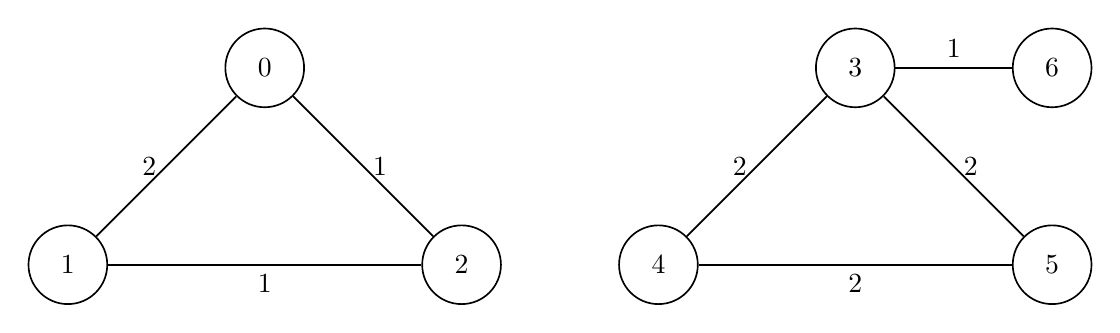
\begin{tikzpicture}[-latex ,auto ,node distance =2.5 cm and 2.5cm ,on grid ,
	semithick ,
	state/.style ={ circle ,top color =white , bottom color = white ,
		draw, black , text=black , minimum width =1 cm}]
		 \node[state] (A) {$0$};
		 \node[state] (B) [below left =of A] {$1$};
		 \node[state] (C) [below right =of A] {$2$};
		 \node[state] (E) [right =of C]{$4$};
		 \node[state] (D) [above right =of E] {$3$};		 
		 \node[state] (F) [below right =of D] {$5$};
		 \node[state] (G) [right =of D]{$6$};
		 \path (A) edge[-] node[left] {$2$} (B); % 0 to 1
		 \path (A) edge[-] node[right] {$1$} (C); % 0 to 2
		 \path (B) edge[-] node[below] {$1$} (C); % 1 to 2
		 \path (D) edge[-] node[left] {$2$} (E); % 3 to 4
		 \path (D) edge[-] node[right] {$2$} (F); % 3 to 5
		 \path (E) edge[-] node[below] {$2$} (F); % 4 to 5
		 \path (D) edge[-] node[above] {$1$} (G); % 3 to 6
	\end{tikzpicture}
	\caption{example graph}
	\label{ex_graph}
\end{figure}
\end{center}

\begin{figure}
	\Tree[.{$\{0,1,2,3,4,5,6\}$\\conn$=0$} 	[.{$\{0,1,2\}$\\conn$=2$} 	[.{$\{0\}$\\conn$=\infty$} ]
												[.{$\{1\}$\\conn$=\infty$} ]
												[.{$\{2\}$\\conn$=\infty$} ]]
								[.{$\{3,4,5,6\}$\\conn$=1$} [.{$\{3,4,5\}$\\conn=4} ]
												[.{$\{6\}$\\conn$=\infty$} ]]]
											
	\caption{decomposition tree for the graph from \cref{ex_graph} for $\alpha=4$}
	\label{ex_decomp_tree}
\end{figure}


\subsection{Algorithm Pseudocode}

\begin{algorithm}
	\caption{insertAndUpdate(a,b)}
	\label{insertAndUpdate}
	\begin{algorithmic}
		\IF {comp[a] == comp[b]}
		\STATE return
		\ENDIF
		\STATE addEdge($a,b$)
		\STATE updateDecomposition$(a,b)$
		\STATE del$\leftarrow$ updateMapping$(alphaConnectedComponents)$
		\STATE delComponents$(del)$
	\end{algorithmic}
\end{algorithm}

\cref{insertAndUpdate} is the main function that is called upon each new request. It checks whether the new request is between different $\alpha$-connected components. If this is not the case it determines that this request can not change the decomposition and returns.

Otherwise the weight of the corresponding edge is increased and other routines are called that update the decomposition based on this new edge.

\cref{updateDecomposition} first determines the smallest sub-graph in the decomposition tree that contains both end points of the request and decomposes this sub-graph. For this decomposition step we use the algorithm proposed by Chang et al. (\cite{Chang2013}). We explain this algorithm in greater detail in \cref{decomp_desc}.

\begin{algorithm}
	\caption{updateDecomposition(a,b)}
	\label{updateDecomposition}
	\begin{algorithmic}
		\STATE q$\leftarrow$ findSmallestSubgraph$(a,b)$
		\WHILE{q not empty}
		\STATE current$\leftarrow$ q.popFront()
		\IF{res.connectivity==alpha}
		\STATE continue
		\ENDIF
		\STATE res$\leftarrow$ decompose(current, current.connectivity+1)//decomposition based on $(s,t)$-cuts
		\STATE current.connectivity $\leftarrow$ value of smallest encountered cut
		\IF {current.connectivity$\geq$alpha}
		\STATE continue
		\ENDIF
		\STATE childrenQueue $\leftarrow$ res
		\STATE //make sure that only subgraphs with higher connectivity are added as children
		\WHILE{childrenQueue not empty}
		\STATE c$\leftarrow$childrenQueue.pop()
		\STATE cRes$\leftarrow$decompose(c, current.connectivity+1)
		\STATE c.connectivity $\leftarrow$ value of smallest encountered cut
		\IF{decompose returned only one graph}
		\STATE current.children.add(cRes)
		\IF{cRes has connectivity smaller than alpha}
		\STATE q.push(cRes)
		\ENDIF
		\ELSE
		\STATE childrenQueue.add(cRes)
		\ENDIF
		\ENDWHILE
		\ENDWHILE
	\end{algorithmic}		
\end{algorithm}

Afterwards the routine \textit{updateMapping} is called which compares the number of components to the number of components before the arrival of the request. Only if the number of components has decreased it checks for the new component as otherwise there was no component merge. 

If there was a merge then the routine checks the size of the newly creted (merged) component and decides whether to delete or to collocate based on the logic described in the previous section.

If a deletion has to be performed then this step is done in the routine \textit{delComponents} (\cref{delComponents}) which resets all edge weights both of edges between nodes of the component as well as all adjacent edges and finally starts the decomposition of the whole graph in order to arrive at a new decomposition that follows the definition from the previous section.

In the case of a collocation the nodes are moved to a cluster that has enough space while updating the reservations and cluster capacities accordingly.



\begin{algorithm}
	\caption{delComponents(del)}
	\label{delComponents}
	\begin{algorithmic}
		\STATE delAllEdges(del)
		\STATE root.connectivity=0
		\STATE root.children=\{\}
		\STATE updateDecomposition(0,1)
	\end{algorithmic}
\end{algorithm}


\begin{comment}
\begin{itemize}
	\item \cref{insertAndUpdate} calls the other routines as needed
	\item \cref{updateDecomposition} starts at the smallest subgraph containing the nodes a and b in the decomposition tree and computes a new decomposition of the subgraph. Specifically it uses the decomposition approach from \cite{Chang2013} to decompose one subgraph and then also computes the subgraphs with the next higher connectivity and recurses until the connectivity has reached alpha.
	\item updateMapping checks whether the alphaConnectedComponents were changed. If yes then it either collocates them if the resulting component is small enough or it adds the component to its return value. Then all the returned components are deleted, i.e. the edges connecting its nodes are deleted and the decomposition is recomputed
	\item this deletion is performed by \cref{delComponents}
\end{itemize}
\end{comment}

\subsection{On the Decomposition of a Subgraph}
\label{decomp_desc}
In this section we describe our algorithm for the decomposition of a given subgraph represented by a node in the decomposition tree. Specifically we describe the general idea behind our implementation of the subroutine \textit{decompose(treeNode, c)} which we have based on the algorithm described by Chang et al. (\cite{Chang2013}). In this algorithm $c$ denotes the connectivity that is to be the basis of this decomposition step.

Given a node $v$ of the decomposition tree, first a \textit{partition graph} is constructed which is a graph consisting of the nodes in the subgraph represented by $v$ and the edges which are between the nodes of the subgraph. This partition graph also supports merges and cuts of its nodes. More specifically the partition graph is initialized as a graph $P=(V,E)$ with $V=nodes(v)$ and $E=\{e=\{u,w\}\in E'|u\in nodes(v)\text{ and }w\in nodes(v)\}$ where $E'$ represents the set of edges in the graph maintained by \crep{}. Additionally we maintain a mapping $M$ which assigns each node from $V$ a set of the nodes in the subgraph represented by the decomposition tree node $v$. Initially M assigns each node in $V$ the subset containing only the node itself.

We now run a \textit{maximum adjacency search} algorithm, sometimes also called \textit{maximum cardinality search} algorithm, (\cite{Stoer1997}) in order to obtain an arbitrary minimum $(s,t)$-cut of the graph.

The maximum adjacency search algorithm is defined as follows: We start with an empty list $L$ to which we add an arbitrary node of $P$. We then continually add the most tightly connected node from $V$ to L, i.e. the node which is connected to the nodes in $L$ via edges of the most total weight. Stoer and Wagner (\cite{Stoer1997}) have shown that the edges between the last two nodes $s$ and $t$ added to $L$ form a minimum $(s,t)$-cut.

We use the value of this cut in order to decide whether to merge the nodes $s$ and $t$ or whether to separate them: if the cut has value less than $c$ we separate the nodes, otherwise we perform a merge.

Here the separation of the nodes $s$ and $t$ means that we remove all edges in the cut from the edges $E$ of the partition graph $P$.

In the case of a merge we combine the nodes s and t and merge the outgoing edges, i.e. we replace the set of nodes $V$ of $P$ by the set $V'=V\backslash\{s,t\}\cup\{v'\}$. The edges $E$ of $P$ are modified by removing all edges adjacent to $s$ and $t$ and adding an edge $e'=\{v',u\}$ of weight $w(\{s,u\})+w(\{t,u\})$ where $w(e)$ denotes the weight of edge $e$ if it exists and is equal to zero otherwise.
Furthermore we adjust the mapping $M$ by setting $M(v')=M(s)\cup M(t)$.

We continually run this algorithm until $P$ contains no edges, i.e. until $E=\emptyset$. The sets of nodes mapped to each ot the nodes of $P$ by $M$ now represent candidate subgraphs for the decomposition. Note though that we have only cut and merged according to minimum $(s,t)$-cuts and not according to minimum cuts. This means that the specific sequence in which we have performed the cuts may influence the result, e.g. if we merged based on a minimum $(s,t)$-cut which is not a minimum cut.

This can be remedied by repeating the procedure on the resulting subgraphs until it returns a subgraph of only one node, i.e. until no separation step is performed during the decomposition. This is due to the fact that Chang et al. (\cite{Chang2013}) have shown that this procedure always cuts a subgraph of connectivity less than $c$ at least once (see Cutability Property in \cite{Chang2013}).

In order to speed up this computation we use the heap data structure proposed and analyzed by Chang et al. (\cite{Chang2013}).

Thus we conclude that this procedure correctly decomposes a given subgraph as Chang et al. have also stated in Theorem 3.1 in \cite{Chang2013}.


\subsection{Running Time}
\label{run_time_sec}
In this section we discuss the polynomial running time of an update of the decomposition tree after a new request has been received in our implementation of \adjDel{}.

\cref{run_time_theo} summarizes our result on the corresponding running time. 

\begin{theo}
	\label{run_time_theo}
	The deterministic algorithm \adjDel{} can be implemented in polynomial time $O(\alpha|V|^2|E|)$.
\end{theo}

\textit{Proof.} The worst case is given when the whole tree has to be recomputed. We first discuss the time complexity of decomposing a single tree node $v$. Let the corresponding subgraph be denoted by $G_v=(V_v, E_v)$.
Since each iteration of the subroutine \textit{decompose} performs at least one cut as long as the connectivity of the given graph is smaller than the current threshold $c$ we conclude that after at most $|V_v|$ iterations of decompose a correct decomposition is found. 

Each step of \textit{decompose} can be performed in $O(|V_v|\cdot|E_v|)$ as the maximum adjacency search algorithm finds an arbitrary minimum $(s,t)$-cut in time $O(|E_v|)$ as shown in theorem 4.1 in \cite{Chang2013} and as there are at most $|V_v|$ minimum $(s,t)$-cuts computed for each invocation of \textit{decompose}.

Hence the complexity of decomposing the subgraph represented by a tree node $v$ is in $O(|V_v|^2|E_v|)$. Let $C_v$ denote the time needed for the decomposition of the subgraph represented  by decomposition tree node $v$.

We now sum this complexity over the nodes for each connectivity level of the decomposition tree. To this end let $level(i)$ denote all nodes in the decomposition tree which are of connectivity exactly $i$.

\begin{align*}
	\sum_{i=0}^{\alpha}\sum_{v\in \text{level}(i)}C_v\leq\sum_{i=0}^{\alpha}O(|V|^2|E|)\in O(\alpha|V|^2|E|).
\end{align*}

We conclude our analysis of the time complexity by observing the polynomial-time complexity of $O(\alpha|V|^2|E|)$.



\section{Evaluation}
In this section we evaluate the quality of the results and the performance of our algorithm implementation by comparing it with several algorithms described in \cref{algSection} on input data sets described in \cref{inputDesc}.

\subsection{Algorithms}
\label{algSection}
We first present the algorithms we compare in order to evaluate our results.

We consider both algorithmic approaches based on maintaining a second-order partition of the nodes into components we discussed in \cref{algIdeas}, i.e. \adjDel{} where on a component deletion all edges inside of and adjacent of the component are deleted and \coreDel{} which only deletes internal edges. Both algorithms start with randomly initialized mappings of nodes to servers.

We have shown the competitive ratio of \adjDel{} in \cref{comp_ratio_theo} and its polynomial running time in the previous section.

We compare these algorithms both with the static graph partitioning algorithm METIS\_PartGraphRecursive implemented in the METIS framework (\cite{Karypis1998, Karypis1998a}) which we will refer to from now on as \static{} and the adaptive/dynamic algorithm \nl{ParMETIS\_V3\_AdaptiveRepart} (\cite{Karypis1999, Schloegel1997, Schloegel2000}) available in the ParMetis framework, referred to as \adapt{}. Both frameworks are known to produce very good results and to be very fast.

We run \adapt{} in an online manner while maintaining a communication graph by inserting an edge or incrementing a corresponding edge weight for each request, i.e. \adapt{} is called after each request is inserted into the graph.

For \static{} we first record the communication graph and give it as input to \static{}. We then compute the cost of \static{} due to migrations from the random initial mapping of nodes to servers and due to remote requests, i.e. the total weight of edges between nodes of the communication graph which \static{} mapped to different servers.

\subsection{Input Data}
\label{inputDesc}

As input data we use several HPC traces (\dbALong{}, \dbBLong{}, \dbCLong{}), the nature of the data is described in more detail by Avin, Ghobadi, Griner and Schmid in \cite{Avin2019}. For the sake of readability we use abbreviations NB for NeckBone and MG for MultiGrid.

All data sets contain 1024 different communication nodes and are limited to the first 300 000 requests. The value of $\alpha$ is set to 6 and the algorithm was tasked to partition the nodes into 32 clusters of size 32 each, i.e. $k=l=32$. The dynamic algorithms are allowed to use augmentation with a factor of $2.1$, i.e. for the dynamic algorithms the maximum cluster capacities are $\lfloor32\cdot2.1\rfloor=67$.

\begin{comment}

\begin{figure}
	\begin{tikzpicture}
	\begin{axis}[
	ybar,
	bar width=1.4cm,
	enlarge x limits=0.25,
	width=\textwidth,
	height=.5\textwidth,
	legend style={at={(0.5,-0.25)},
		anchor=north,legend columns=-1},
	symbolic x coords={A,B,C,D},
	xtick=data,
	xlabel={input set},
	nodes near coords,
	nodes near coords align={vertical},
	ymin=0,ymax=370000,
	ylabel={cost},
	]
	\addplot table[x=database,y=decomposition]{\totalcostplot};
	\addplot table[x=database,y=ParMetis]{\totalcostplot};
	\addplot table[x=database, y=Static]{\totalcostplot};
	\legend{Decomposition, ParMetis, Static}
	\end{axis}
	\end{tikzpicture}
	\caption{comparison of total cost}\label{totalCostPlot}
\end{figure}

\begin{figure}
	\begin{tikzpicture}
	\begin{axis}[
	ybar,
	bar width=1.4cm,
	enlarge x limits=0.25,
	width=\textwidth,
	height=.5\textwidth,
	legend style={at={(0.5,-0.25)},
		anchor=north,legend columns=-1},
	symbolic x coords={A,B,C,D},
	xtick=data,
	xlabel={input set},
	nodes near coords,
	nodes near coords align={vertical},
	ymin=0,ymax=750000,
	ylabel={time in ms},
	]
	\addplot table[x=database,y=decomposition]{\runtimeplot};
	\addplot table[x=database,y=ParMetis]{\runtimeplot};
	\addplot table[x=database, y=Static]{\runtimeplot};
	\legend{Decomposition, ParMetis, Static}
	\end{axis}
	\end{tikzpicture}
	\caption{comparison of run time}\label{runTimePlot}
\end{figure}

\end{comment}

\subsection{Comparison of \adjDel{} and \coreDel{}}

We compare the results of \adjDel{} and \coreDel{} first. \cref{costPlotCrep} shows the resulting total cost of both algorithms on the different input sets as well as how this cost is split between communication and migration costs. One can see that \adjDel{} always produces better results, especially for the second and third input set. 

We now discuss the differences of the two algorithms in terms of communication and migration cost. The figures illustrate that \adjDel{} pays only very slightly less for communication requests than \coreDel{} whereas the former pays significantly reduced migration cost. This suggests that that the deletion of adjacent edges indeed improves the quality of the results by reducing the number of migrations. 

Finally \cref{runTimePlotCrep} compares the running times of both algorithms. One can see that \adjDel{} performs drastically better than \coreDel{} in this regard. This may be due to the fact that \adjDel{} deletes edges more frequently and thus needs to take less edges into account when updating the decomposition tree.

Also note that both algorithms pay generally more for migrations than for communication. This suggests that there may be room for fine-tuning these algorithms in order achieve a more balanced distribution of the cost. One such adjustment is investigated in the next section, namely whether we can improve the results by changing the algorithms in such a way that they only merge once a connectivity of $2\cdot\alpha$ is reached.

\begin{figure}
	\begin{tikzpicture}
	\begin{axis}[
	ybar stacked,
	bar width=1cm,
	enlarge x limits=0.25,
	width=.45\textwidth,
	height=.5\textwidth,
	legend style={at={(0.5,-0.25)},
		anchor=north,legend columns=-1},
	symbolic x coords={\dbA,\dbB,\dbC},
	xtick=data,
	xlabel={input set},
	%nodes near coords,
	%nodes near coords align={vertical},
	ymajorgrids=true,
	ymin=0,ymax=370000,
	ylabel={cost},
	]
	\addplot table[x=database,y=AdjDel]{\commcostplot};
	\addplot table[x=database,y=AdjDel]{\migcostplot};
	%\legend{communication cost, migration cost}
	\end{axis}
	
	\begin{axis}[
	ybar stacked,
	bar width=1cm,
	enlarge x limits=0.25,
	width=.45\textwidth,
	height=.5\textwidth,
	legend style={at={(-0.2,-0.25)},
		anchor=north,legend columns=-1},
	symbolic x coords={\dbA,\dbB,\dbC},
	xtick=data,
	xlabel={input set},
	xshift=7cm,
	%nodes near coords,
	%nodes near coords align={vertical},
	ymajorgrids=true,
	ymin=0,ymax=370000,
	ylabel={cost},
	]
	\addplot table[x=database,y=CoreDel]{\commcostplot};
	\addplot table[x=database,y=CoreDel]{\migcostplot};
	\legend{communication cost, migration cost}
	\end{axis}
	\end{tikzpicture}
	\caption{comparison of the total cost of \adjDel{} (left) and \coreDel{} (right)}\label{costPlotCrep}
\end{figure}


\begin{comment}
	

\begin{figure}
	\begin{tikzpicture}
	\begin{axis}[
	ybar=7pt,
	bar width=1.4cm,
	enlarge x limits=0.25,
	width=\textwidth,
	height=.5\textwidth,
	legend style={at={(0.5,-0.25)},
		anchor=north,legend columns=-1},
	symbolic x coords={A,B,C},
	xtick=data,
	xlabel={input set},
	nodes near coords,
	nodes near coords align={vertical},
	ymin=0,ymax=370000,
	ylabel={cost},
	]
	\addplot table[x=database,y=AdjDel]{\totalcostplot};
	\addplot table[x=database,y=CoreDel]{\totalcostplot};
	\legend{\adjDel{}, \coreDel{}}
	\end{axis}
	\end{tikzpicture}
	\caption{comparison of the total cost of \adjDel{} and \coreDel{}}\label{totalCostPlotCrep}
\end{figure}

\begin{figure}
	\begin{tikzpicture}
	\begin{axis}[
	ybar=7pt,
	bar width=1.4cm,
	enlarge x limits=0.25,
	width=\textwidth,
	height=.5\textwidth,
	legend style={at={(0.5,-0.25)},
		anchor=north,legend columns=-1},
	symbolic x coords={A,B,C},
	xtick=data,
	xlabel={input set},
	nodes near coords,
	nodes near coords align={vertical},
	ymin=0,ymax=370000,
	ylabel={cost},
	]
	\addplot table[x=database,y=AdjDel]{\commcostplot};
	\addplot table[x=database,y=CoreDel]{\commcostplot};
	\legend{\adjDel{}, \coreDel{}}
	\end{axis}
	\end{tikzpicture}
	\caption{comparison of the communication cost of \adjDel{} and \coreDel{}}\label{commCostPlotCrep}
\end{figure}

\begin{figure}
	\begin{tikzpicture}
	\begin{axis}[
	ybar=7pt,
	bar width=1.4cm,
	enlarge x limits=0.25,
	width=\textwidth,
	height=.5\textwidth,
	legend style={at={(0.5,-0.25)},
		anchor=north,legend columns=-1},
	symbolic x coords={A,B,C},
	xtick=data,
	xlabel={input set},
	nodes near coords,
	nodes near coords align={vertical},
	ymin=0,ymax=370000,
	ylabel={cost},
	]
	\addplot table[x=database,y=AdjDel]{\migcostplot};
	\addplot table[x=database,y=CoreDel]{\migcostplot};
	\legend{\adjDel{}, \coreDel{}}
	\end{axis}
	\end{tikzpicture}
	\caption{comparison of the migration cost of \adjDel{} and \coreDel{}}\label{migCostPlotCrep}
\end{figure}
\end{comment}

\begin{figure}
	\begin{tikzpicture}
	\begin{axis}[
	ybar=7pt,
	bar width=1.4cm,
	enlarge x limits=0.25,
	width=\textwidth,
	height=.5\textwidth,
	legend style={at={(0.5,-0.25)},
		anchor=north,legend columns=-1},
	symbolic x coords={\dbA,\dbB,\dbC},
	xtick=data,
	xlabel={input set},
	nodes near coords,
	nodes near coords align={vertical},
	ymin=0,ymax=700000,
	ylabel={time [ms]},
	]
	\addplot table[x=database,y=AdjDel]{\runtimeplot};
	\addplot table[x=database,y=CoreDel]{\runtimeplot};
	\legend{\adjDel{}, \coreDel{}}
	\end{axis}
	\end{tikzpicture}
	\caption{comparison of running time of \adjDel{} and \coreDel{}}\label{runTimePlotCrep}
\end{figure}

\subsection{On the Influence of the Connectivity Threshold}
\label{alphaInf}

In the previous section we observed that both \coreDel{} and \adjDel{} have higher migration cost than communication cost. This leads to the question whether we can find adjustments that allow us to achieve a better balance of the different costs. In this section we investigate the influence of the connectivity threshold which determines when components are merged. Up until this point it was set to $\alpha$. As we show there lies potential in adjusting this threshold in order to improve the quality of the solution. 

Namely we discuss the results of both algorithms for the case where they only merge components once a connectivity of at least $2\cdot\alpha$ is reached. Note that this only affects the analysis by constant factors, namely the statements from \cref{cut_lemma} and \cref{cut_lemma_upper} are multiplied by a factor of two. This may only impact the other cost bounds by a factor of two which leaves our bound on the competitive ratio of \adjDel{} unaffected.

\cref{costPlotCrepTwoAlpha} shows the total cost of \adjDel{} and \coreDel{} for this scenario. One can see that the cost of both algorithms is reduced, but \coreDel{} has improved significantly more than \adjDel{}.

When looking at the distribution of this cost to communication and migration costs one can see that now the communication costs of both algorithms is higher than the migration cost in all cases. For \coreDel{} this has improved the balance of both costs, but \adjDel{} now has significantly higher communication cost than migration cost. This suggests that by adjusting the exact value of connectivity at which these algorithms perform their merges one might be able to further improve the quality of the results. It may even be possible to adjust this parameter dynamically based on some data gathered as requests are processed.

These improvements come at a cost of running time as \cref{runTimePlotCrep2A} shows, almost doubling or tripling the times of the previous results in some cases. Especially the already worse run times of \coreDel{} are drastically increased.

\begin{figure}
	\begin{tikzpicture}
	\begin{axis}[
	ybar stacked,
	bar width=1cm,
	enlarge x limits=0.25,
	width=.45\textwidth,
	height=.5\textwidth,
	legend style={at={(0.5,-0.25)},
		anchor=north,legend columns=-1},
	symbolic x coords={\dbA,\dbB,\dbC},
	xtick=data,
	xlabel={input set},
	%nodes near coords,
	%nodes near coords align={vertical},
	ymajorgrids=true,
	ymin=0,ymax=370000,
	ylabel={cost},
	]
	\addplot table[x=database,y=AdjDelDouble]{\commcostplotTwoAlpha};
	\addplot table[x=database,y=AdjDelDouble]{\migcostplotTwoAlpha};
	%\legend{communication cost, migration cost}
	\end{axis}
	
	\begin{axis}[
	ybar stacked,
	bar width=1cm,
	enlarge x limits=0.25,
	width=.45\textwidth,
	height=.5\textwidth,
	legend style={at={(-0.2,-0.25)},
		anchor=north,legend columns=-1},
	symbolic x coords={\dbA,\dbB,\dbC},
	xtick=data,
	xlabel={input set},
	xshift=7cm,
	%nodes near coords,
	%nodes near coords align={vertical},
	ymajorgrids=true,
	ymin=0,ymax=370000,
	ylabel={cost},
	]
	\addplot table[x=database,y=CoreDelDouble]{\commcostplotTwoAlpha};
	\addplot table[x=database,y=CoreDelDouble]{\migcostplotTwoAlpha};
	\legend{communication cost, migration cost}
	\end{axis}
	\end{tikzpicture}
	\caption{comparison of the total cost of \adjDel{} (left) and \coreDel{} (right) in the case where merges are performed at connectivity $2\cdot\alpha$}\label{costPlotCrepTwoAlpha}
\end{figure}

\begin{comment}
	
\begin{figure}
	\begin{tikzpicture}
	\begin{axis}[
	ybar=7pt,
	bar width=1.4cm,
	enlarge x limits=0.25,
	width=\textwidth,
	height=.5\textwidth,
	legend style={at={(0.5,-0.25)},
		anchor=north,legend columns=-1},
	symbolic x coords={A,B,C},
	xtick=data,
	xlabel={input set},
	nodes near coords,
	nodes near coords align={vertical},
	ymin=0,ymax=370000,
	ylabel={cost},
	]
	\addplot table[x=database,y=AdjDelDouble]{\totalcostplotTwoAlpha};
	\addplot table[x=database,y=CoreDelDouble]{\totalcostplotTwoAlpha};
	\legend{\adjDel{}, \coreDel{}}
	\end{axis}
	\end{tikzpicture}
	\caption{comparison of the total cost of \adjDel{} and \coreDel{} in the case where merges are performed at connectivity $2\cdot\alpha$}\label{totalCostPlotCrep2A}
\end{figure}

\begin{figure}
	\begin{tikzpicture}
	\begin{axis}[
	ybar=7pt,
	bar width=1.4cm,
	enlarge x limits=0.25,
	width=\textwidth,
	height=.5\textwidth,
	legend style={at={(0.5,-0.25)},
		anchor=north,legend columns=-1},
	symbolic x coords={A,B,C},
	xtick=data,
	xlabel={input set},
	nodes near coords,
	nodes near coords align={vertical},
	ymin=0,ymax=370000,
	ylabel={cost},
	]
	\addplot table[x=database,y=AdjDelDouble]{\commcostplotTwoAlpha};
	\addplot table[x=database,y=CoreDelDouble]{\commcostplotTwoAlpha};
	\legend{\adjDel{}, \coreDel{}}
	\end{axis}
	\end{tikzpicture}
	\caption{comparison of the communication cost of \adjDel{} and \coreDel{} in the case where merges are performed at connectivity $2\cdot\alpha$}\label{commCostPlotCrep2A}
\end{figure}

\begin{figure}
	\begin{tikzpicture}
	\begin{axis}[
	ybar=7pt,
	bar width=1.4cm,
	enlarge x limits=0.25,
	width=\textwidth,
	height=.5\textwidth,
	legend style={at={(0.5,-0.25)},
		anchor=north,legend columns=-1},
	symbolic x coords={A,B,C},
	xtick=data,
	xlabel={input set},
	nodes near coords,
	nodes near coords align={vertical},
	ymin=0,ymax=370000,
	ylabel={cost},
	]
	\addplot table[x=database,y=AdjDelDouble]{\migcostplotTwoAlpha};
	\addplot table[x=database,y=CoreDelDouble]{\migcostplotTwoAlpha};
	\legend{\adjDel{}, \coreDel{}}
	\end{axis}
	\end{tikzpicture}
	\caption{comparison of the migration cost of \adjDel{} and \coreDel{} in the case where merges are performed at connectivity $2\cdot\alpha$}\label{migCostPlotCrep2A}
\end{figure}
\end{comment}

\begin{figure}
	\begin{tikzpicture}
	\begin{axis}[
	ybar=7pt,
	bar width=1.4cm,
	enlarge x limits=0.25,
	width=\textwidth,
	height=.5\textwidth,
	legend style={at={(0.5,-0.25)},
		anchor=north,legend columns=-1},
	symbolic x coords={\dbA,\dbB,\dbC},
	xtick=data,
	xlabel={input set},
	nodes near coords,
	nodes near coords align={vertical},
	ymin=0,ymax=1100000,
	ylabel={time [ms]},
	]
	\addplot table[x=database,y=AdjDelDouble]{\runtimeplotTwoAlpha};
	\addplot table[x=database,y=CoreDelDouble]{\runtimeplotTwoAlpha};
	\legend{\adjDel{}, \coreDel{}}
	\end{axis}
	\end{tikzpicture}
	\caption{comparison of running time of \adjDel{} and \coreDel{} in the case where merges are performed at connectivity $2\cdot\alpha$}\label{runTimePlotCrep2A}
\end{figure}



\begin{comment}
We will first discuss the overall results of our experiments, i.e. we will describe the quality of the results (see \cref{totalCostPlot}) as well as the running time needed for each examined algorithm (see \cref{runTimePlot}).\nl
The static algorithm is shown to give the best results in the shortest time, but the low running was also to be expected as it is only called once as opposed to the 300 000 times the other algorithms need to decide whether they want to change their partitioning. The static algorithm also has knowledge of all requests and as a result is able to produce the best results. \nl
For data set A our decomposition algorithm beats the adaptive ParMetis algorithm by a significant amount of about one third of the cost of the latter while ParMetis is significantly faster. For data sets B and C ParMetis is shown to produce slightly better results within drastically less computation time. It is worth mentioning that ParMetis uses the ... graph description format that does not allow for easy adaptation on the fly and needed to be recomputed after every request during our tests. However, we chose not to include this in the running time calculations.\nl
	

\begin{figure}
	\begin{tikzpicture}
	\begin{axis}[
	ybar,
	bar width=1.4cm,
	enlarge x limits=0.25,
	width=\textwidth,
	height=.5\textwidth,
	legend style={at={(0.5,-0.25)},
		anchor=north,legend columns=-1},
	symbolic x coords={A,B,C,D},
	xtick=data,
	xlabel={input set},
	nodes near coords,
	nodes near coords align={vertical},
	ymin=0,ymax=200000,
	ylabel={cost},
	]
	\addplot table[x=database,y=decomposition]{\commcostplot};
	\addplot table[x=database,y=ParMetis]{\commcostplot};
	\addplot table[x=database, y=Static]{\commcostplot};
	\legend{Decomposition, ParMetis, Static}
	\end{axis}
	\end{tikzpicture}
	\caption{comparison of communication cost}\label{commCostPlot}
\end{figure}

\begin{figure}
	\begin{tikzpicture}
	\begin{axis}[
	ybar,
	bar width=1.4cm,
	enlarge x limits=0.25,
	width=\textwidth,
	height=.5\textwidth,
	legend style={at={(0.5,-0.25)},
		anchor=north,legend columns=-1},
	symbolic x coords={A,B,C,D},
	xtick=data,
	xlabel={input set},
	nodes near coords,
	nodes near coords align={vertical},
	ymin=0,ymax=370000,
	ylabel={cost},
	]
	\addplot table[x=database,y=decomposition]{\migcostplot};
	\addplot table[x=database,y=ParMetis]{\migcostplot};
	\addplot table[x=database, y=Static]{\migcostplot};
	\legend{Decomposition, ParMetis, Static}
	\end{axis}
	\end{tikzpicture}
	\caption{comparison of migration cost}\label{migCostPlot}
\end{figure}

In the next section we discuss the general distribution of the total costs of each algorithm to communication (see \cref{commCostPlot}) and migration costs (\cref{migCostPlot}).\nl
Both ParMetis as well as our decomposition algorithm produce significantly more migration cost than communication cost while the static algorithm predominantly pays for communication. This shows that the dynamic algorithms tend to migrate too much while the static implementation is restricted to only migrate once to a static configuration it finds suitable and as a result has to pay more for communication. This also shows that there is potential to refine the dynamic implementations in such a way that they produce more balanced, and hopefully also less, cost overall.

\end{comment}

\subsection{Results of \adapt{} and \static}

\begin{figure}
	\begin{tikzpicture}
	\begin{axis}[
	ybar stacked,
	bar width=1cm,
	enlarge x limits=0.25,
	width=.45\textwidth,
	height=.5\textwidth,
	legend style={at={(0.5,-0.25)},
		anchor=north,legend columns=-1},
	symbolic x coords={\dbA,\dbB,\dbC},
	xtick=data,
	xlabel={input set},
	%nodes near coords,
	%nodes near coords align={vertical},
	ymajorgrids=true,
	ymin=0,ymax=370000,
	ylabel={cost},
	]
	\addplot table[x=database,y=Adaptive]{\commcostplot};
	\addplot table[x=database,y=Adaptive]{\migcostplot};
	%\legend{communication cost, migration cost}
	\end{axis}
	
	\begin{axis}[
	ybar stacked,
	bar width=1cm,
	enlarge x limits=0.25,
	width=.45\textwidth,
	height=.5\textwidth,
	legend style={at={(-0.2,-0.25)},
		anchor=north,legend columns=-1},
	symbolic x coords={\dbA,\dbB,\dbC},
	xtick=data,
	xlabel={input set},
	xshift=7cm,
	%nodes near coords,
	%nodes near coords align={vertical},
	ymajorgrids=true,
	ymin=0,ymax=370000,
	ylabel={cost},
	]
	\addplot table[x=database,y=Static]{\commcostplot};
	\addplot table[x=database,y=Static]{\migcostplot};
	\legend{communication cost, migration cost}
	\end{axis}
	\end{tikzpicture}
	\caption{comparison of the total cost of \adapt{} (left) and \static{} (right)}\label{costPlotMetis}
\end{figure}

\begin{comment}
	
\begin{figure}
	\begin{tikzpicture}
	\begin{axis}[
	ybar=7pt,
	bar width=1.4cm,
	enlarge x limits=0.25,
	width=\textwidth,
	height=.5\textwidth,
	legend style={at={(0.5,-0.25)},
		anchor=north,legend columns=-1},
	symbolic x coords={A,B,C},
	xtick=data,
	xlabel={input set},
	nodes near coords,
	nodes near coords align={vertical},
	ymin=0,ymax=370000,
	ylabel={cost},
	]
	\addplot table[x=database,y=Adaptive]{\totalcostplot};
	\addplot table[x=database,y=Static]{\totalcostplot};
	\legend{\adapt{}, \static{}}
	\end{axis}
	\end{tikzpicture}
	\caption{comparison of the total cost of \adapt{} and \static{}}\label{totalCostPlotMetis}
\end{figure}

\begin{figure}
	\begin{tikzpicture}
	\begin{axis}[
	ybar=7pt,
	bar width=1.4cm,
	enlarge x limits=0.25,
	width=\textwidth,
	height=.5\textwidth,
	legend style={at={(0.5,-0.25)},
		anchor=north,legend columns=-1},
	symbolic x coords={A,B,C},
	xtick=data,
	xlabel={input set},
	nodes near coords,
	nodes near coords align={vertical},
	ymin=0,ymax=370000,
	ylabel={cost},
	]
	\addplot table[x=database,y=Adaptive]{\commcostplot};
	\addplot table[x=database,y=Static]{\commcostplot};
	\legend{\adapt{}, \static{}}
	\end{axis}
	\end{tikzpicture}
	\caption{comparison of the communication cost of \adapt{} and \static{}}\label{commCostPlotMetis}
\end{figure}

\begin{figure}
	\begin{tikzpicture}
	\begin{axis}[
	ybar=7pt,
	bar width=1.4cm,
	enlarge x limits=0.25,
	width=\textwidth,
	height=.5\textwidth,
	legend style={at={(0.5,-0.25)},
		anchor=north,legend columns=-1},
	symbolic x coords={A,B,C},
	xtick=data,
	xlabel={input set},
	nodes near coords,
	nodes near coords align={vertical},
	ymin=0,ymax=370000,
	ylabel={cost},
	]
	\addplot table[x=database,y=Adaptive]{\migcostplot};
	\addplot table[x=database,y=Static]{\migcostplot};
	\legend{\adapt{}, \static{}}
	\end{axis}
	\end{tikzpicture}
	\caption{comparison of the migration cost of \adapt{} and \static{}}\label{migCostPlotMetis}
\end{figure}
\end{comment}

\begin{figure}
	\begin{tikzpicture}
	\begin{axis}[
	ybar=7pt,
	bar width=1.4cm,
	enlarge x limits=0.25,
	width=\textwidth,
	height=.5\textwidth,
	legend style={at={(0.5,-0.25)},
		anchor=north,legend columns=-1},
	symbolic x coords={\dbA,\dbB,\dbC},
	xtick=data,
	xlabel={input set},
	nodes near coords,
	nodes near coords align={vertical},
	ymin=0,ymax=150000,
	ylabel={time [ms]},
	]
	\addplot table[x=database,y=Adaptive]{\runtimeplot};
	\addplot table[x=database,y=Static]{\runtimeplot};
	\legend{\adapt{}, \static{}}
	\end{axis}
	\end{tikzpicture}
	\caption{comparison of running time of \adapt{} and \static{}}\label{runTimePlotMetis}
\end{figure}

\cref{costPlotMetis} shows the total cost of the solutions of \adapt{} and \static{}. One can see that \static{} is able to produce results that far surpass \adapt{}. In fact the results of \static{} are also a significant improvement over the results of \adjDel{} and \coreDel{} presented before. But it is also important to note that \static{} is only useful in scenarios where the communication patterns and frequencies stay mostly the same over time. Otherwise the approach to record the communication graph and then use \static{} in order to compute a partitioning may lead to consistent results. 

We stress that the implementations of \static{} and \adapt{} rely on heuristics only and do not provide any guarantees while we have shown that our algorithm \adjDel{} is a competitive algorithm with competitive ratio $O(2/\epsilon\cdot k\log k)$.

Finally \cref{runTimePlotMetis} illustrates the run times of \adapt{} and \static{}. Note that static is only run once on the communication graph after all requests have been revealed which means that it is expected for \static{} to have the fastest running time. But also \adapt{} achieves faster running times than our dynamic implementations.

%\clearpage

\section{Conclusion}
We have discussed different ideas for component-based algorithms for the Dynamic Balanced Graph Partitioning Problem as well as the corresponding implications and challenges for the competitive analysis. 

We have shown that our algorithm \adjDel{} has a competitive ratio of $O(2/\epsilon\cdot k\log k)$ and we have presented our decomposition-based approach to its implementation. 

Finally we have evaluated the results of our implementation by comparing it with three other algorithms: \coreDel{} which is a variation of \adjDel{} which deletes fewer edges and \adapt{} and \static{} which are available via METIS and ParMETIS frameworks, respectively. Furthermore we have explored the possibility of making slight adaptations of our algorithms in order to improve their results.

\section{Future Work}
Even though we have already shown very promising results as to the overall performance of our algorithms together with theoretical guarantees there are still areas in which our work could be expanded upon.

As discussed in \cref{alphaInf} we see great potential in making adjustments to our algorithms, especially \coreDel{}, in order to improve their results even further while also preserving our result on the competitive ratio.

Such adjustments may be achieved for example by changing certain algorithm parameters such as the connectivity threshold

There may also be potential in adapting and improving our decomposition tree data structure in order to improve running times.

One such avenue for improvement may be to parallelize the computation of the decomposition of disjoint subgraphs. This could be both used to handle multiple requests in parallel if they only affect disjoint sub-graphs, i.e. their corresponding trees do not overlap in the decomposition tree, as well as in order to speed up the computation of the decomposition the children trees during the update process after a new request has been received by \crep{}.

\clearpage %move references to the back
\addcontentsline{toc}{section}{References}
\bibliographystyle{plain}
\bibliography{../../Dropbox/ThesisPapers/ThesisBibTex}                             

	
\end{document}
